\documentclass[english,11pt]{beamer}

\DeclareMathOperator{\Cov}{Cov}
\DeclareMathOperator{\Var}{Var}
\DeclareMathOperator{\E}{\mathbb{E}}
\DeclareMathOperator{\Proba}{\mathbb{P}}

\newcommand{\Covb}[2]{\ensuremath{\Cov\!\left[#1,#2\right]}}
\newcommand{\Eb}[1]{\ensuremath{\E\!\left[#1\right]}}
\newcommand{\Pb}[1]{\ensuremath{\Proba\!\left[#1\right]}}
\newcommand{\Varb}[1]{\ensuremath{\Var\!\left[#1\right]}}

% norm
\newcommand{\norm}[1]{\| #1 \|}

\newcommand{\indep}{\rotatebox[origin=c]{90}{$\models$}}





\usepackage{mathptmx,amsmath,amssymb,graphicx,bibentry,bbm,babel,ragged2e}

\makeatletter

\newcommand{\noun}[1]{\textsc{#1}}
\newcommand{\jitem}[1]{\item \begin{justify} #1 \end{justify} \vfill{}}
\newcommand{\sframe}[2]{\frame{\frametitle{#1} #2}}

\newenvironment{centercolumns}{\begin{columns}[c]}{\end{columns}}
%\newenvironment{jitem}{\begin{justify}\begin{itemize}}{\end{itemize}\end{justify}}

\usetheme{Warsaw}
\setbeamertemplate{footline}[text line]{}
\setbeamercolor{structure}{fg=purple!50!blue, bg=purple!50!blue}

\setbeamersize{text margin left=15pt,text margin right=15pt}

\setbeamercovered{transparent}


\@ifundefined{showcaptionsetup}{}{%
 \PassOptionsToPackage{caption=false}{subfig}}
\usepackage{subfig}

\usepackage[utf8]{inputenc}
\usepackage[T1]{fontenc}


\usepackage{multirow}


\makeatother

\begin{document}

% Modeling Urban Morphogenesis: towards an integration of territories and networks

%%%%%%%%%
% Abstract

%



\title{Modeling Network Morphogenesis: a co-evolution approach}

\author{J.~Raimbault$^{1,2,\ast}$\\
\texttt{juste.raimbault@iscpif.fr}
}


\institute{$^{1}$UPS CNRS 3611 ISCPIF\\
$^{2}$UMR CNRS 8504 G{\'e}ographie-cit{\'e}s
}


\date{FMR Seminar\\\smallskip
May 2nd 2018
}

\frame{\maketitle}





%%%%%%%%%%%%%%%%%%%
%% ABSTRACT
%\textbf{Keywords : }\textit{Urban and Network Morphogenesis Modeling ; Interactions between Networks and Territories ; Co-evolution}


% Cette présentation sera l'occasion de discuter des objectifs de la modélisation en analyse de réseaux. Elle proposera un cadre théorique situant la croissance des réseaux dans un contexte de co-évolution au sein des systèmes territoriaux, et illustrera la mise en place de modèles stylisés et sur données empiriques, incluant par exemple la multi-modélisation de la croissance du réseau routier par divers processus complémentaires allant de l'auto-organisation biologique aux analyses coût-bénéfices ou à la rupture de potentiel. 

%Une autre illustration décrira une modélisation endogène des processus de gouvernance de l'évolution des réseaux de transport, couplée à un modèle d'usage du sol pour former un modèle de co-évolution.






%%%%%%%%%%%%%%%%%
%\section{Introduction}
%%%%%%%%%%%%%%%%%



\sframe{Complex processes of Urban Morphogenesis}{

\centering

% center of Paris
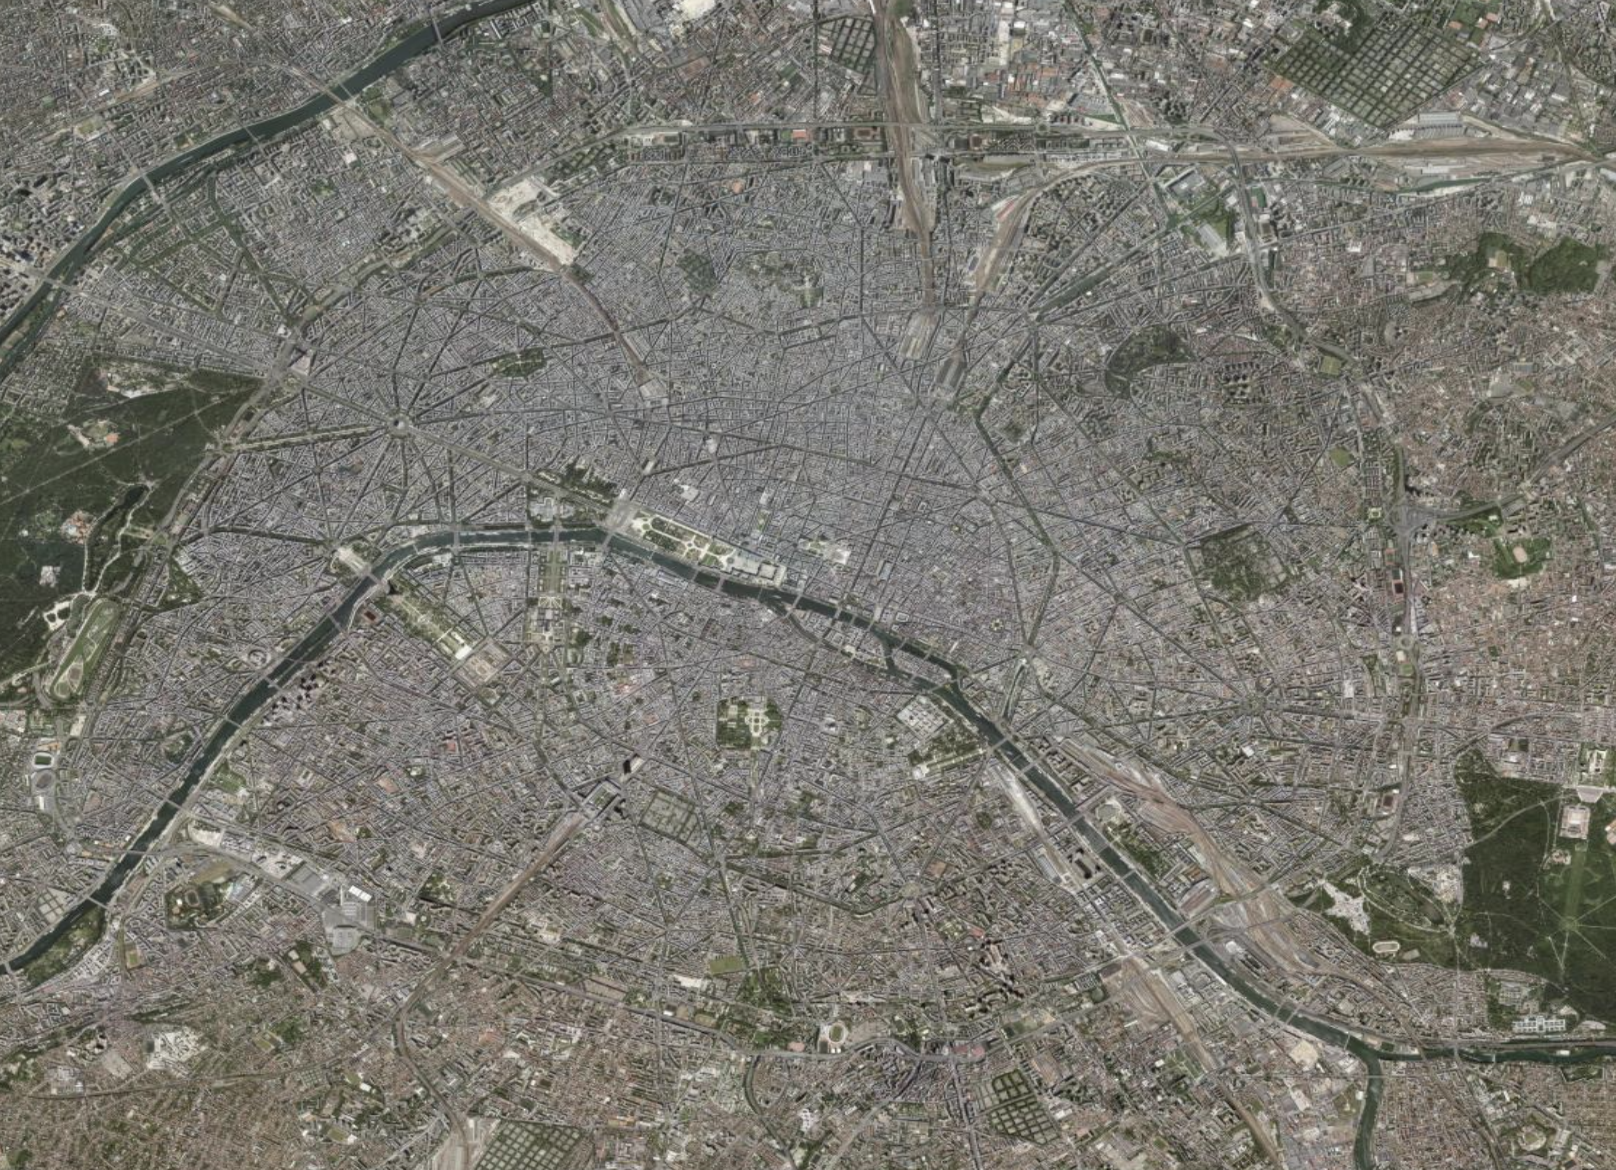
\includegraphics[width=0.9\textwidth]{figures/intro_paname}

\footnotesize\textit{Source: Geoportail}
}

\sframe{Complex processes of Urban Morphogenesis}{

\centering

% large bp
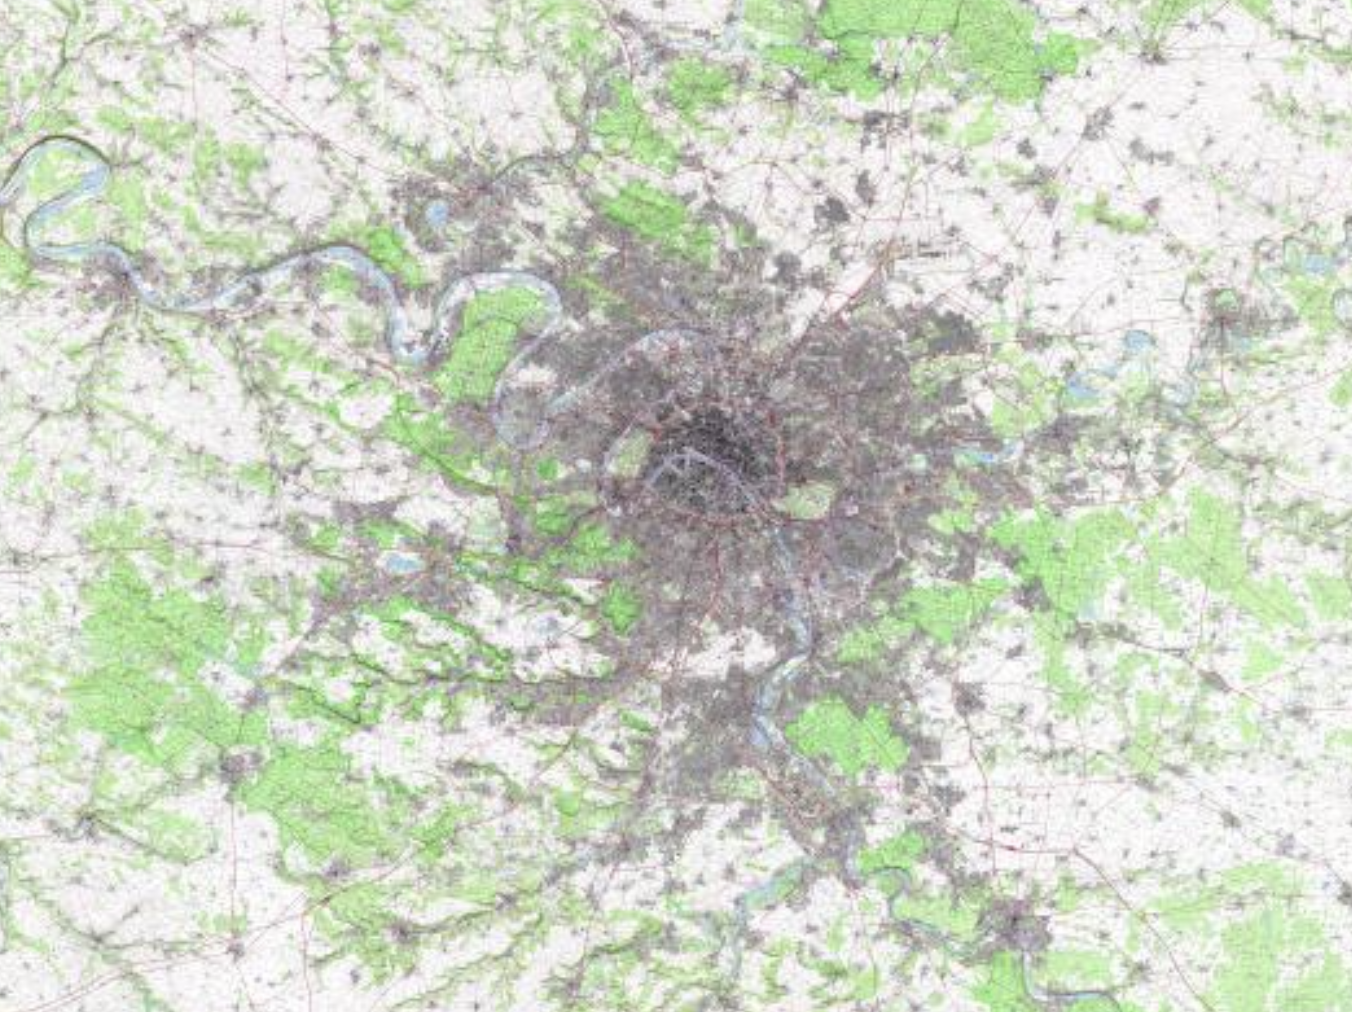
\includegraphics[width=0.9\textwidth]{figures/intro_bp}

\footnotesize\textit{Source: Geoportail}
}



\sframe{What is Morphogenesis ?}{

\textbf{Morphogenesis} (\textit{Oxford dictionary}) 
\begin{enumerate}
\item \textit{Biology} : The origin and development of morphological characteristics
\item \textit{Geology} : The formation of landforms or other structures.
\end{enumerate}

\bigskip

\textbf{History of the notion}

$\rightarrow$ Started significantly with embryology around 1930~\cite{abercrombie1977concepts} 

$\rightarrow$ Turing's 1952 paper~\cite{turing1952chemical}, linked to the development of Cybernetics

$\rightarrow$ first use in 1871, large peak in usage between 1907-1909, increase until 1990, decrease until today. \textit{Scientific fashion ?}


}



\sframe{Modeling Urban Morphogenesis}{

\textit{More or less explicit use of the concept of Morphogenesis in Urban Simulation, depending on the scale and the approach.}

\medskip
                                                                                                                                                                                                                                                                                                                                                                                                                                                                                                                                                                                                        
\begin{itemize}
	\item \cite{makse1998modeling} correlated growth
	\item \cite{10.1371/journal.pone.0133780} multi-scale migration and percolation
	\item \cite{bonin2012modele} qualitative differentiation of urban function
	\item \cite{achibet2014model} procedural model at the micro-scale
	\item \cite{caruso2011morphological} micro-economic model of sprawl
	\item \cite{bonin2014modelisation} urban economics morphogenesis, only work to explicitly mention the morphogen
\end{itemize}


}



\sframe{Examples}{

\begin{figure}
\subfloat[Microeconomic model of sprawl, \cite{caruso2011morphological}]{
%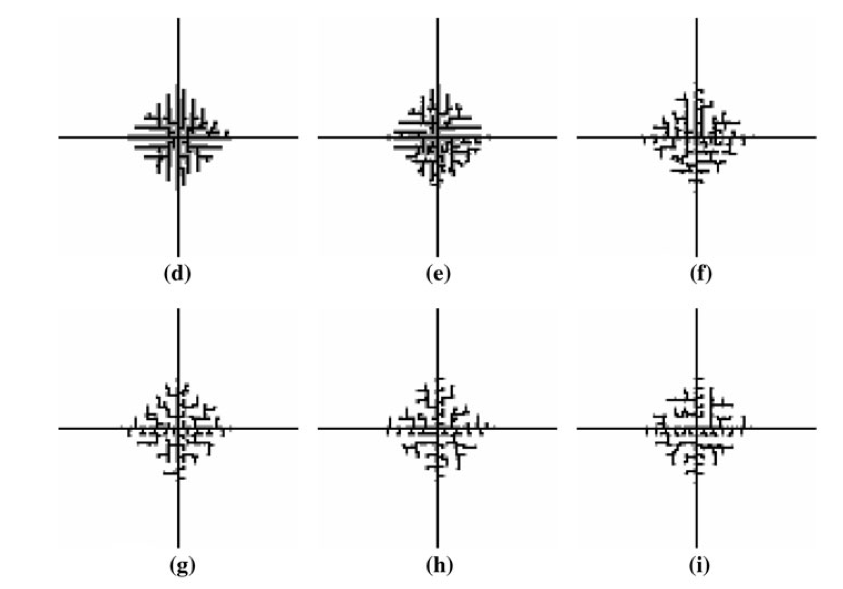
\includegraphics[trim=5cm 0cm 0cm 7cm,scale=0.23]{figures/rbd_dbmexample}}
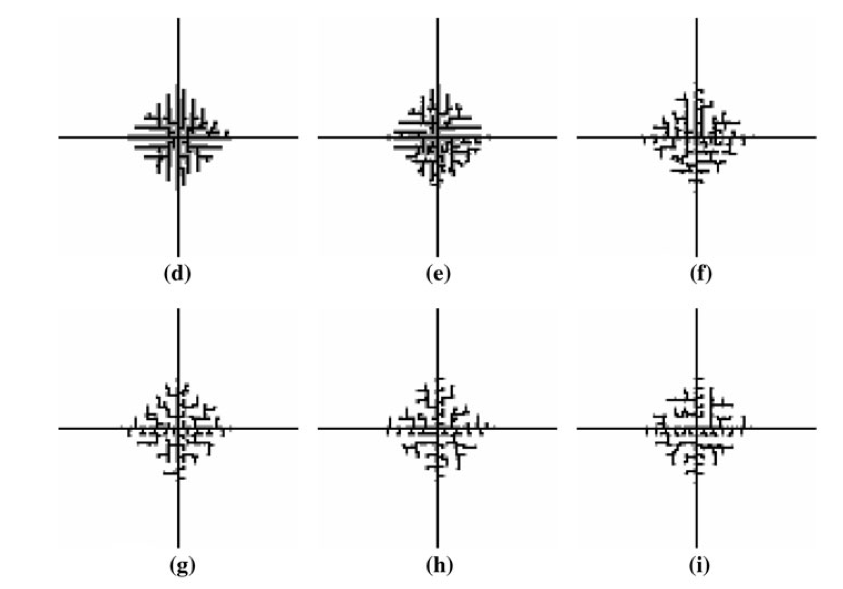
\includegraphics[scale=0.23]{figures/rbd_dbmexample}}
\subfloat[Land use simulations, \cite{van2012activity}]{
%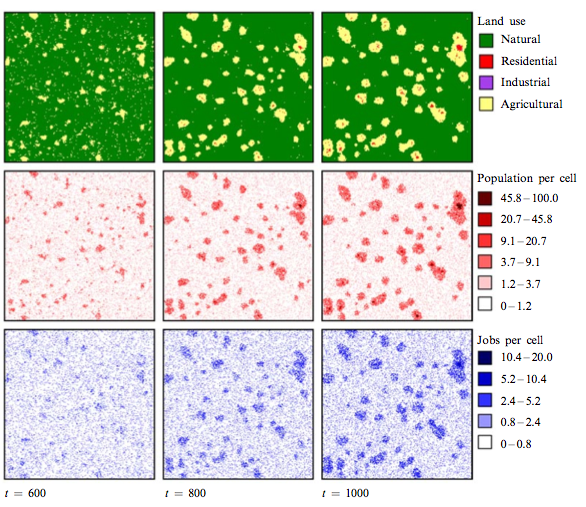
\includegraphics[trim=0cm 0cm 0cm 7cm,scale=0.27]{figures/rbd_exampleWhite}}
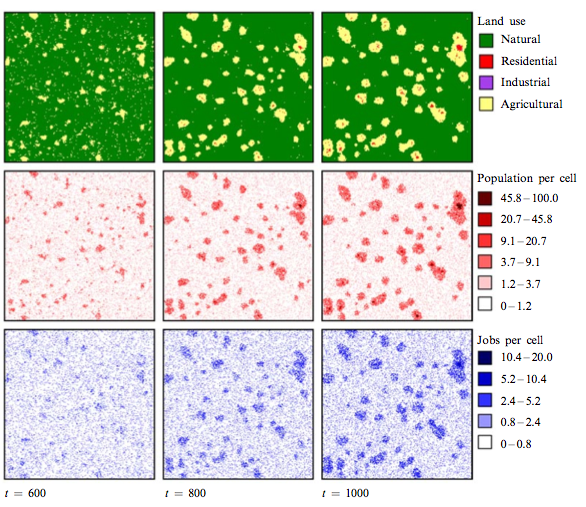
\includegraphics[scale=0.27]{figures/rbd_exampleWhite}}
\end{figure}


%\cite{peeters2009space} 1D CA to show path-dependence of settlements patterns

}


%
%\sframe{CA in Urban Planning}{
%\begin{itemize}
%\vfill{}
%
%\item \begin{justify}First introduction for reproduction of fractal urban form and land-use patterns in \cite{white1993cellular,batty1997cellular}.\end{justify}
%\vfill{}
%\item \begin{justify}Since then, numerous applications, e.g. coupling with GIS in quantitative
%geography, calibration on real land-use configurations (review in
%\cite{iltanen2012cellular}).\end{justify}
%\vfill{}
%\item \begin{justify}Examples: \cite{DBM11} micro-economic model of sprawl; \cite{peeters2009space} 1D CA to show
%path-dependence of settlements patterns;
%\cite{Wu96alinguistic} real-time rules for sustainable development.\end{justify}
%\end{itemize}
%}







%\sframe{Which models for Urban Morphogenesis ?}{

% why modeling, exemple of rbd
% -> champ ; difficultés ("verrous". rq : j'aime pas la metaphore du verrou, trop cadrant et suppose que deja construit et qu'il suffit d'ouvrir. demarche epistemo de co-evol des connaissances, ni inductif ni deductif. il faut contruire. horizons d'exploration plus appropriés. rejoint l'idee de faire rentrer dans "cadre analytique" : cases prédéfinies, alors qu'il s'agit au contraire de définir ces cases. -> relire hdr arnaud

%\justify

%The relation between the form and the function is a crucial feature in Urban Morphogenesis models.

%\bigskip

%$\rightarrow$\textit{At the crossroad between Urban Simulation and Artificial Life, few models try to integrate and explain the link between Urban Form and Function}

%\medskip

%$\rightarrow$\textit{Importance of parcimonious, stylized models: modeling as a tool to understand processes}


%\bigskip

%\textbf{Research Objective : } Explore simple models to capture morphogenesis based on abstract representation of urban processes; test their ability to reproduce existing urban systems or to optimize new systems from scratch

%}



\sframe{Territorial approach to networks}{

% context theorique Dupuy

The relation between the form and the function is a crucial feature in Urban Morphogenesis models.

\medskip

$\rightarrow$ Networks as realized potential transactions (Dupuy's territorial theory of networks \cite{dupuy1987vers}).

\medskip

$\rightarrow$ Networks capture functions within co-evolution processes with territories, and the study of network morphogenesis thus informs more generally on urban morphogenesis.

\medskip

$\rightarrow$ Importance of parcimonious, stylized models: modeling as a tool to understand processes.


}





\sframe{Different approaches to Network Morphogenesis}{

\vspace{-1cm}
\textit{Different models with different ontologies and coupling ontologies}

\bigskip
\bigskip

%\setlength{\columnseprule}{0.4pt}

\begin{columns}
\begin{column}{0.50\textwidth}
\centering\textit{Network}
\end{column}
%\vrule{}
%\vrule{}
\begin{column}{0.50\textwidth}
\centering\textit{Co-evolution}
\end{column}
\end{columns}

\bigskip

\begin{columns}
\begin{column}{0.25\textwidth}
\centering
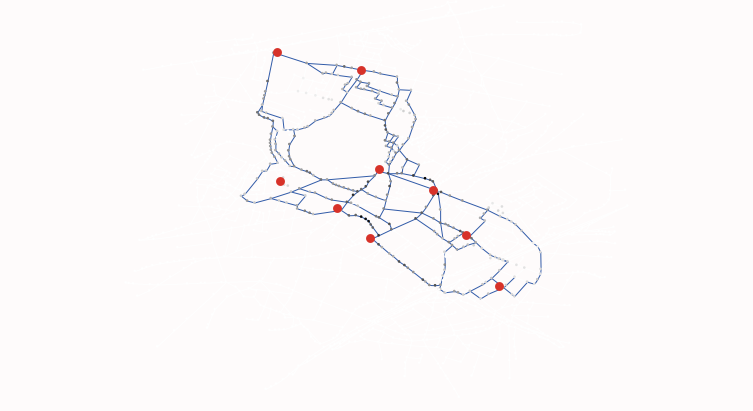
\includegraphics[width=\textwidth]{figures/slimemould_reseauFinal}

\footnotesize\textit{Self-organizing biological network}

\medskip

\it\textbf{Optimisation}

\end{column}

\vspace*{-1cm}\vrule{}
\begin{column}{0.25\textwidth}
\centering
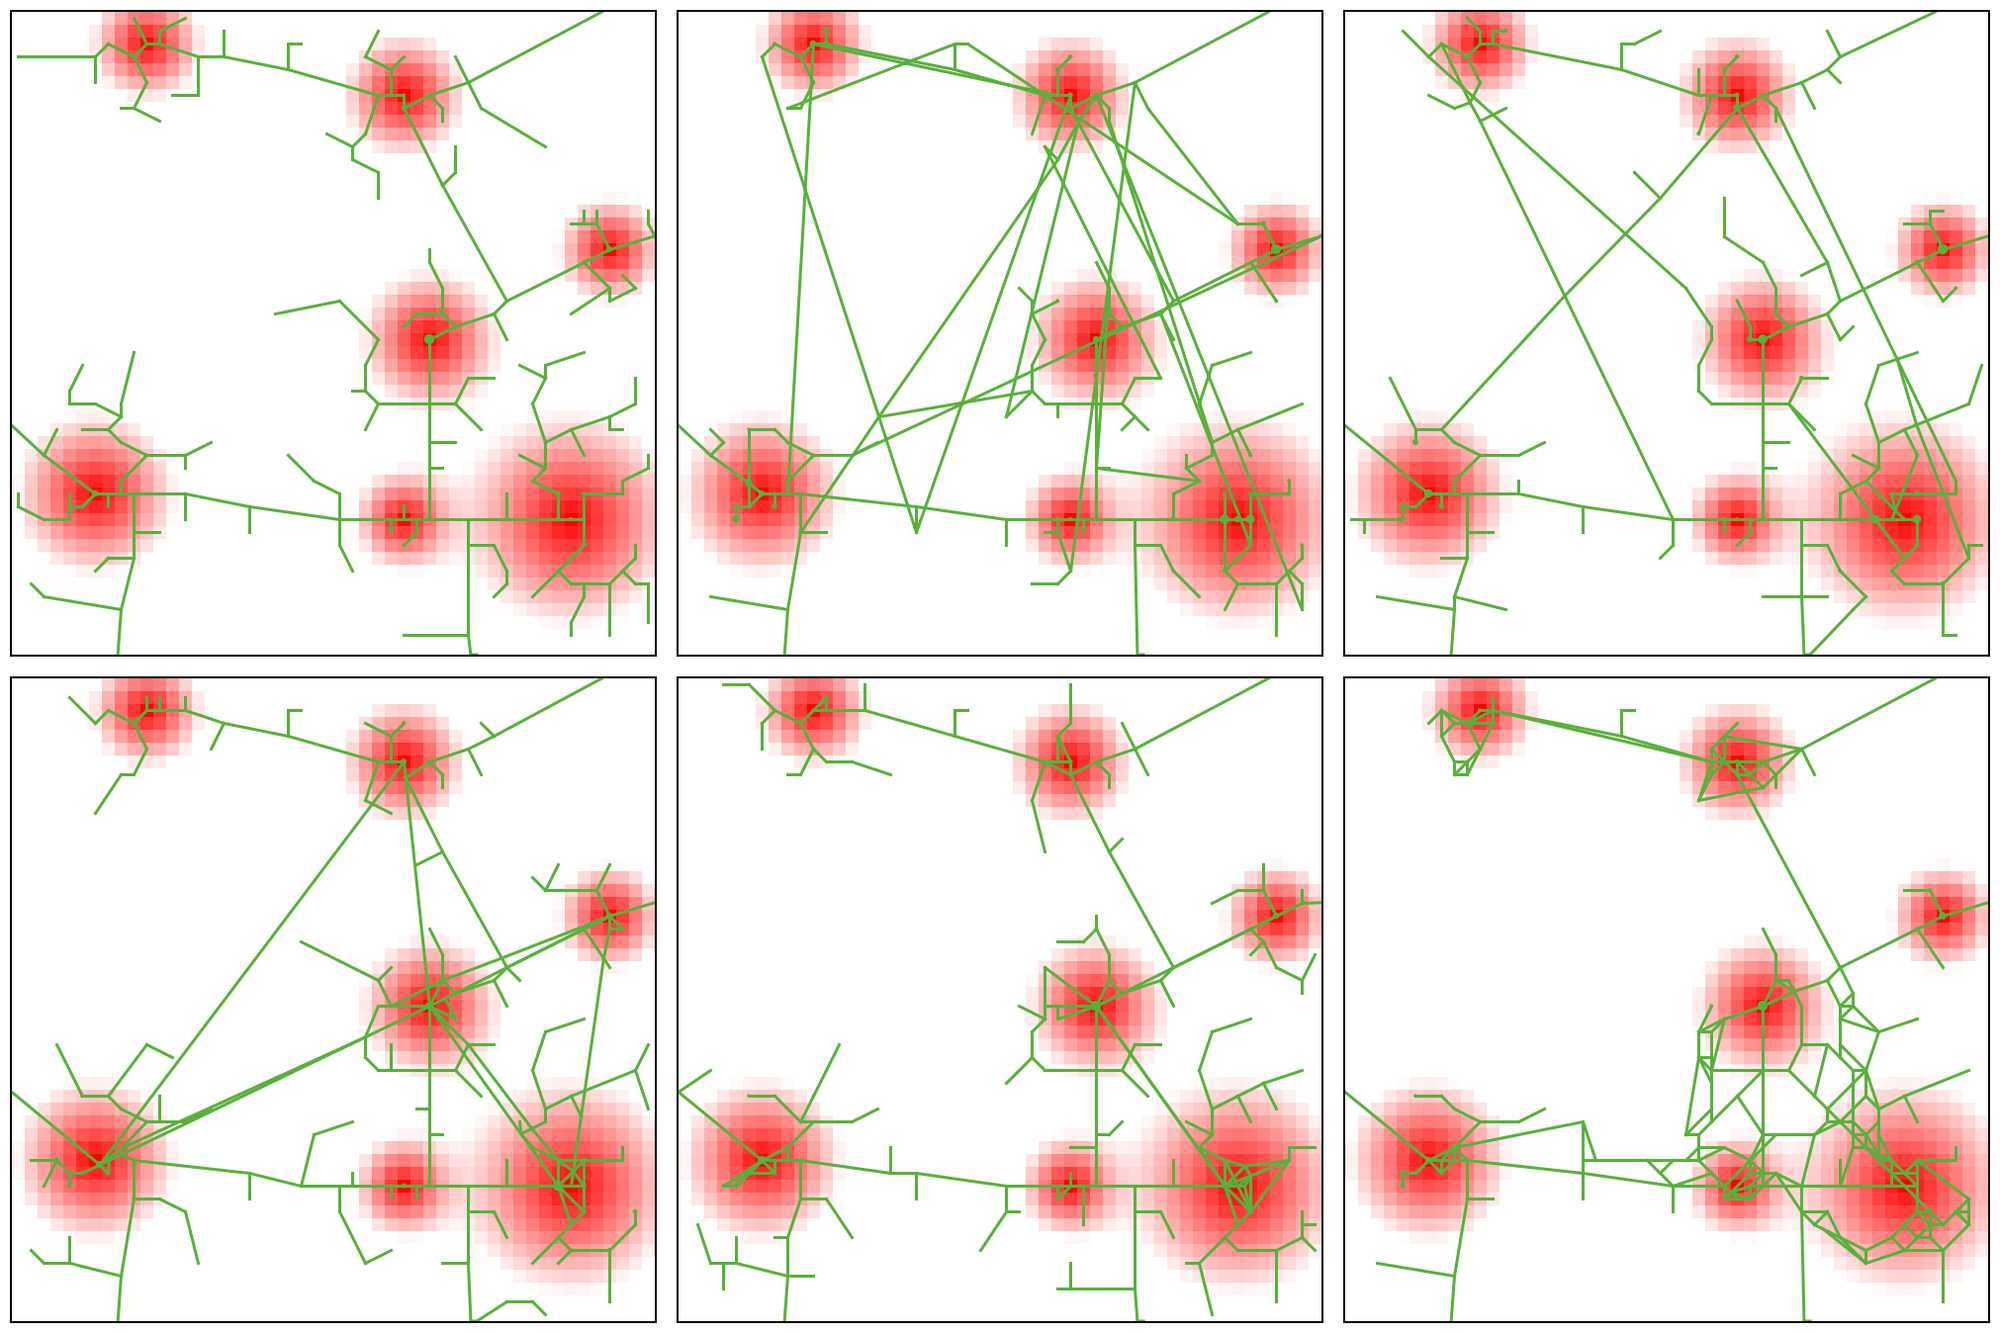
\includegraphics[width=\columnwidth]{figures/7-1-2-fig-networkgrowth-examples.jpg}

\footnotesize\textit{Multi-modeling network growth}
%
\medskip
%
\it\textbf{Explication}
\end{column}

\vrule{}
\begin{column}{0.25\textwidth}
\centering
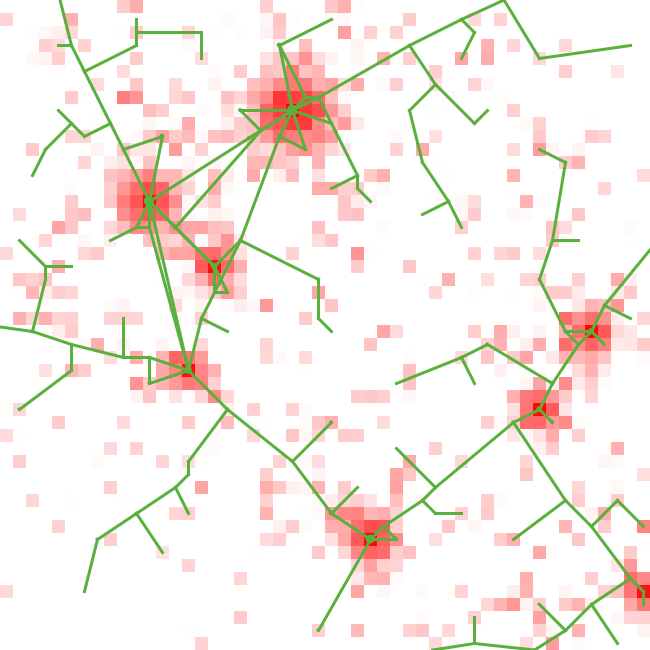
\includegraphics[width=\textwidth]{figures/coevol_example_nw-cost}\\

\footnotesize\textit{Co-evolution model}

\medskip

\it\textbf{Explication}

\end{column}
\vrule{}
\begin{column}{0.25\textwidth}
\centering
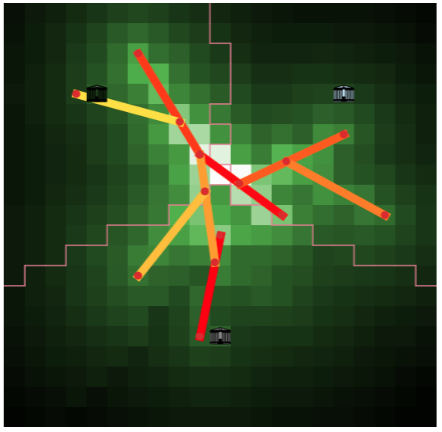
\includegraphics[width=\textwidth]{figures/lutetia_longtimelimit_2.png}\\

\footnotesize\textit{Transportation governance}

\medskip

\it\textbf{Explication}

\end{column}
\end{columns}

%\setlength{\columnseprule}{0pt}

}





%%%%%%%%%%%%%%%%%%%%
%%%% Network Morphogenesis



\sframe{Network morphogenesis model}{

Model studied by~\cite{tero2010rules} : exploration and reinforcement by a slime mould searching for ressources

\medskip

Settings :
\begin{itemize}
	\item Initial homogeneous network of tubes $ij$ of length $L_{ij}$, variable diameter $D_{ij}$, carrying a flow $Q_{ij}$.
	\item Nodes $i$ with a pressure $p_i$.
	\item $N$ nodes are origin/destination points : randomly at each step one becomes source $p_{i_+}=I_0$ and one other sink $p_{i_-}=-I_0$
\end{itemize}


}

\sframe{Network evolution}{

At each iteration :
\begin{enumerate}
	\item Determination of flows with Kirchoff's law (electrostatic analogy) : Ohm's law $Q_{ij}=\frac{D_{ij}}{L_{ij}}\cdot(p_{i}-p_{j})$ and conservation of flows $\sum_{j\rightarrow i}Q_{ij} = 0 , \sum_{j\rightarrow i_\pm}Q_{i_{\pm}j} = \pm I_0$
	\item Evolution of diameters ($\gamma$ reinforcement parameter) by
	\[
	\frac{dD_{ij}}{dt}=\frac{\left|Q_{ij}\right|^{\gamma}}{1+\left|Q_{ij}\right|^{\gamma}}-D_{ij}
	\]
\end{enumerate}

\medskip


$\rightarrow$ Extraction of the final network after convergence given a threshold parameter for diameters %(bimodal final distributions)

\medskip

$\rightarrow$ Multi-scale model : diameters are constant during an iteration to obtain equilibrium flows

}



\sframe{Indicators}{

Behavior of the model evaluated with performance indicators for generated network $(V_f,E_f)$, that are contradictory objectives :
          \bigskip
          \begin{itemize}
          \item Construction costs $c=\sum_{ij\in E_f}D_{ij}(t_f)$
          \bigskip
          \item \begin{justify}Average performance~\cite{banos2012towards}
          \[
          v=\frac{1}{|V_f|^2}\sum_{i,j\in V_f}\frac{d_{i\rightarrow j}}{||\vec{i}-\vec{j}||}
          \]
          \end{justify}
          \bigskip
          \item Robustness (\textit{Network Trip Robustness} index~\cite{sullivan2010identifying})
          \end{itemize}

}



\sframe{Example of networks}{
 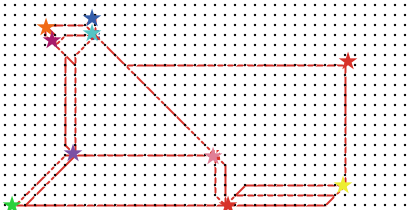
\includegraphics[width=0.48\textwidth]{figures/slimemould_networkDense}
 \hfill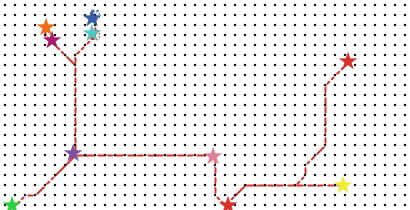
\includegraphics[width=0.48\textwidth]{figures/slimemould_networkLessDense}\\
          \bigskip
 \justify
          \textit{Sensitivity of network topology to reinforcement coefficient $\gamma$. Left : $\gamma \sim 1$, robust network. Right : $\gamma >> 1$, arborescent network.}
}




\sframe{Sensitivity analysis}{
 
          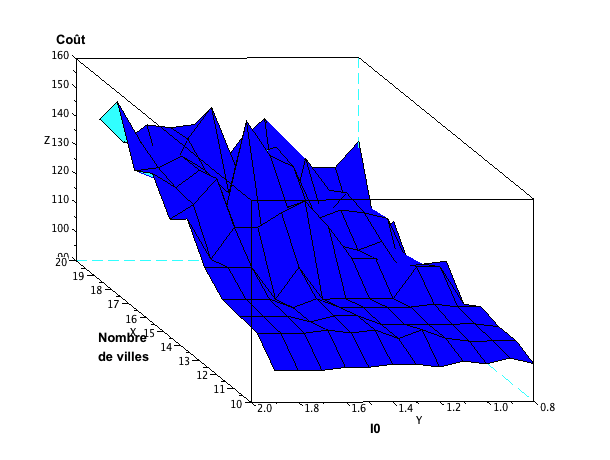
\includegraphics[width=0.5\textwidth]{figures/slimemould_graphe_cout}
          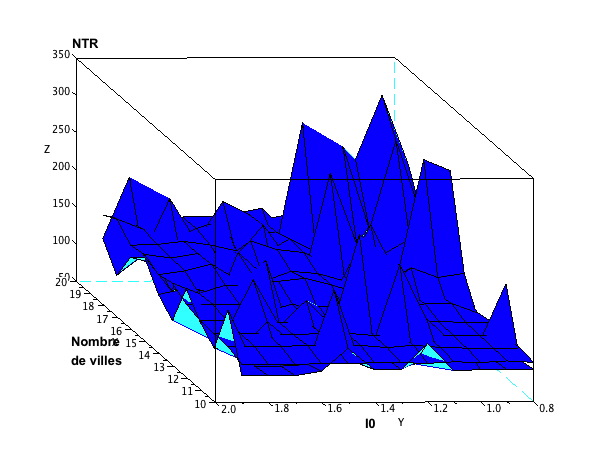
\includegraphics[width=0.5\textwidth]{figures/slimemould_graphe_NTR}\\
          \bigskip
          \textit{Sensitivity of indicators to parameters $(N,I_0)$.}
      
}





\sframe{Application : Optimal transportation Corridor}{
          
Abstract application : \textit{Given a distribution of nodes to serve (sinks), what is the optimal corridor for an infrastructure at a larger scale (train or metro) for which stations are sources, in the sense of the multi-objective optimality of the local self-organized network ?}

\medskip
          
$\rightarrow$ Heuristic exploration of an arborescent set of potential infrastructures

\medskip

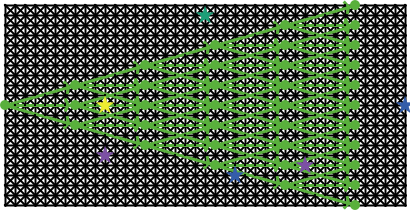
\includegraphics[width=0.48\textwidth]{figures/slimemould_implantationtree}
\hfill 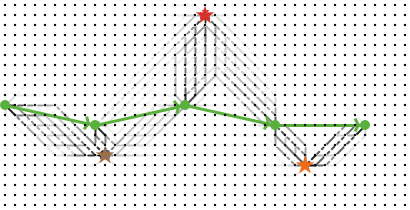
\includegraphics[width=0.48\textwidth]{figures/slimemould_ImplantationTreeview}
         	
%\textit{Heuristic tree to explore infrastructures.}
%\textit{Example of network generation for a given infrastructure.} 
          
}
          
          
          
\sframe{Pareto Optimisation}{
          
%\centering
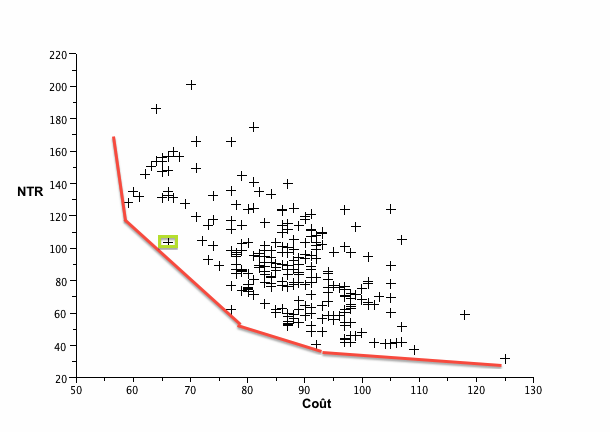
\includegraphics[width=0.48\textwidth]{figures/slimemould_implantationcntr}
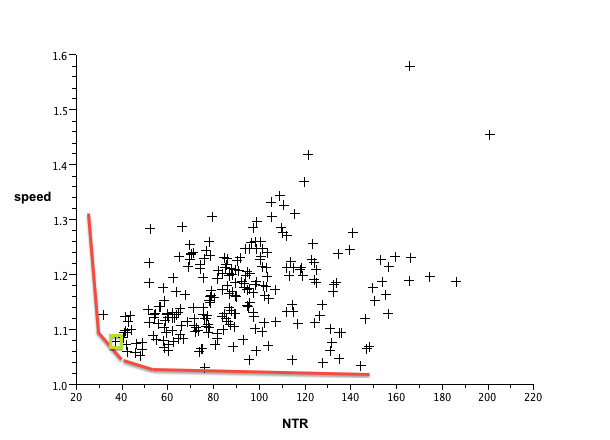
\includegraphics[width=0.48\textwidth]{figures/slimemould_implantationntrspeed}
          
\textit{Pareto optimisation : projection of explored configurations in indicator space to obtain the Pareto front.}          
}

\sframe{Pareto Optimisation}{

\centering
  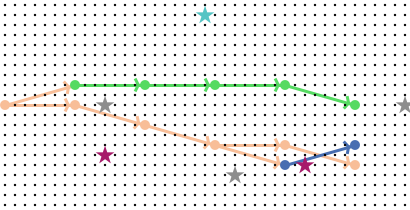
\includegraphics[width=0.8\textwidth]{figures/slimemould_paretosimplantation}

\medskip

\textit{Configurations corresponding to three optimal points.}

}


\sframe{Application : Optimal Network Design}{

\footnotesize

$\rightarrow$ Mission of prospective for Romainville city : itinary of an intra-urban shuttle with imposed stops.

\medskip

$\rightarrow$ NP-hard problem similar to a Travelling Salesman Problem, but multi-objective (cost, speed, robustness). The bottom-up network generation applied on the initial street network gives a compromise solution.

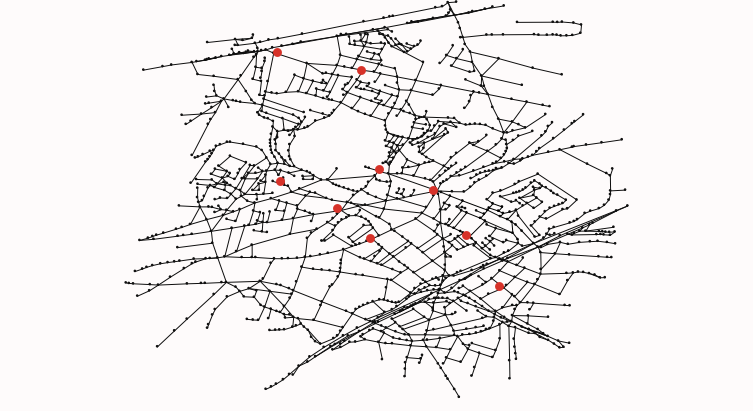
\includegraphics[width=0.32\columnwidth]{figures/slimemould_tick1}
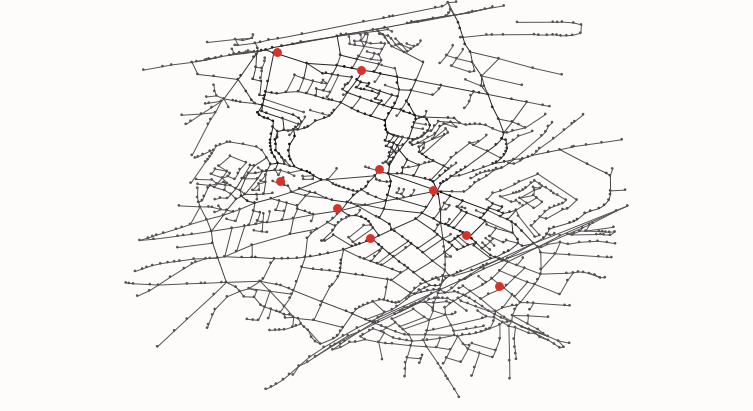
\includegraphics[width=0.32\columnwidth]{figures/slimemould_tick10}
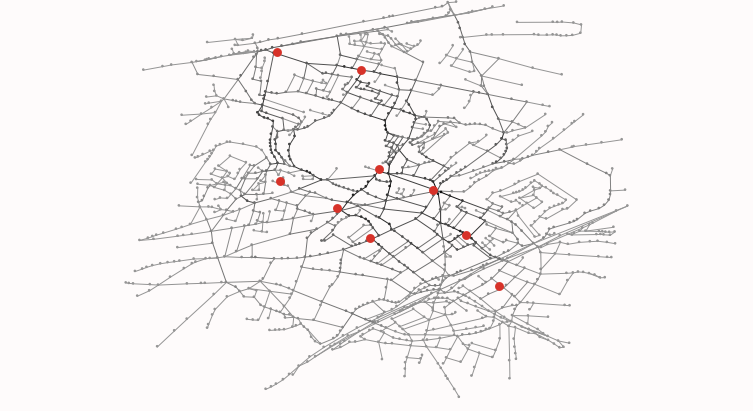
\includegraphics[width=0.32\columnwidth]{figures/slimemould_tick20}\\
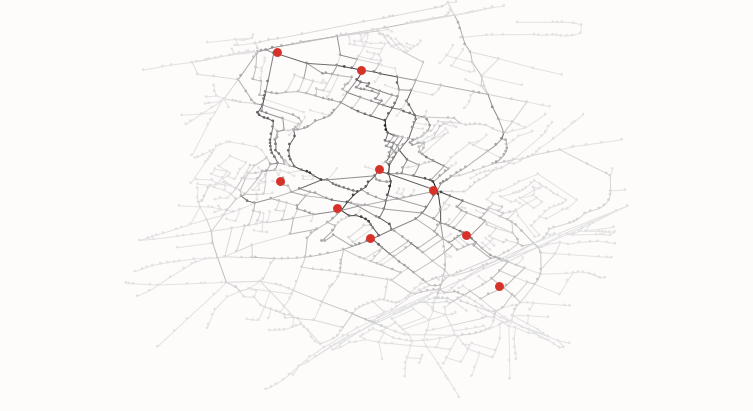
\includegraphics[width=0.32\columnwidth]{figures/slimemould_tick50}
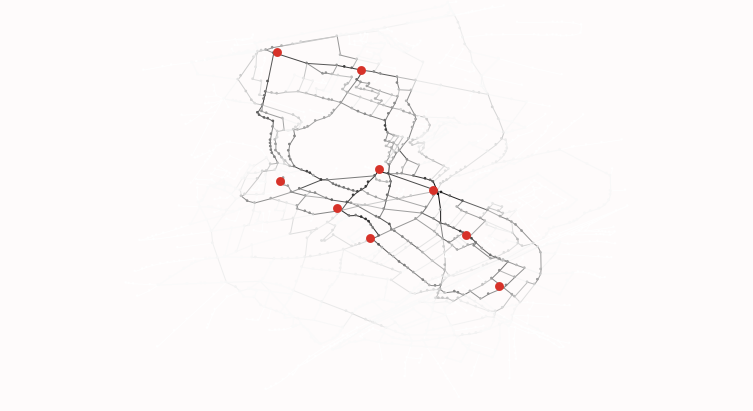
\includegraphics[width=0.32\columnwidth]{figures/slimemould_tick101}
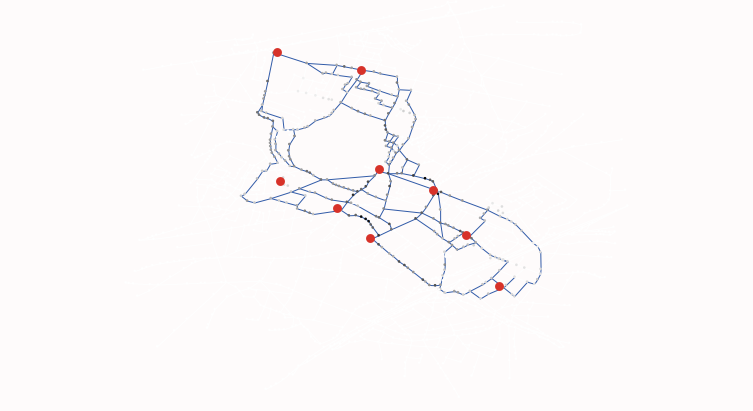
\includegraphics[width=0.32\columnwidth]{figures/slimemould_reseauFinal}\\

\textit{Progressive convergence of the network towards an optimal network connecting the fixed points (in red), starting from the initial street network.}

}





\sframe{Including more complex processes ?}{

% transition : representation of territories

\textit{Which ontology to include more complex functional properties ?}

\medskip

$\rightarrow$ Territorial systems as the strong coupling between territories and (potential and realized) networks \cite{dupuy1987vers}.

\medskip

$\rightarrow$ Networks convey functional notions of centralities and accessibility, among others ; have furthermore proper topological properties.


}


\sframe{Interactions between Networks and Territories}{

% qualitative slide
% eventually layus on literature with the cit nw ? maybe too much
% def. covevol : besoin coevol regimes, annexe
% idem macrocoevol en annexe


\textit{Complex co-evolutive processes between Territories and Transportation Networks}

\medskip

\centering

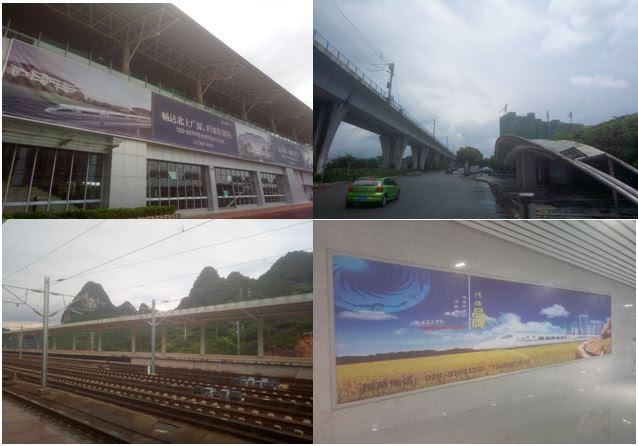
\includegraphics[height=0.7\textheight]{figures/intro_fieldwork}

\footnotesize

\textit{Expanding HSR network in China and ambiguous effects (Source : fieldwork survey)}


}









%\sframe{Causality regimes between network and density variables}{


%\begin{columns}

%\column{0.65\textwidth}
%\centering
%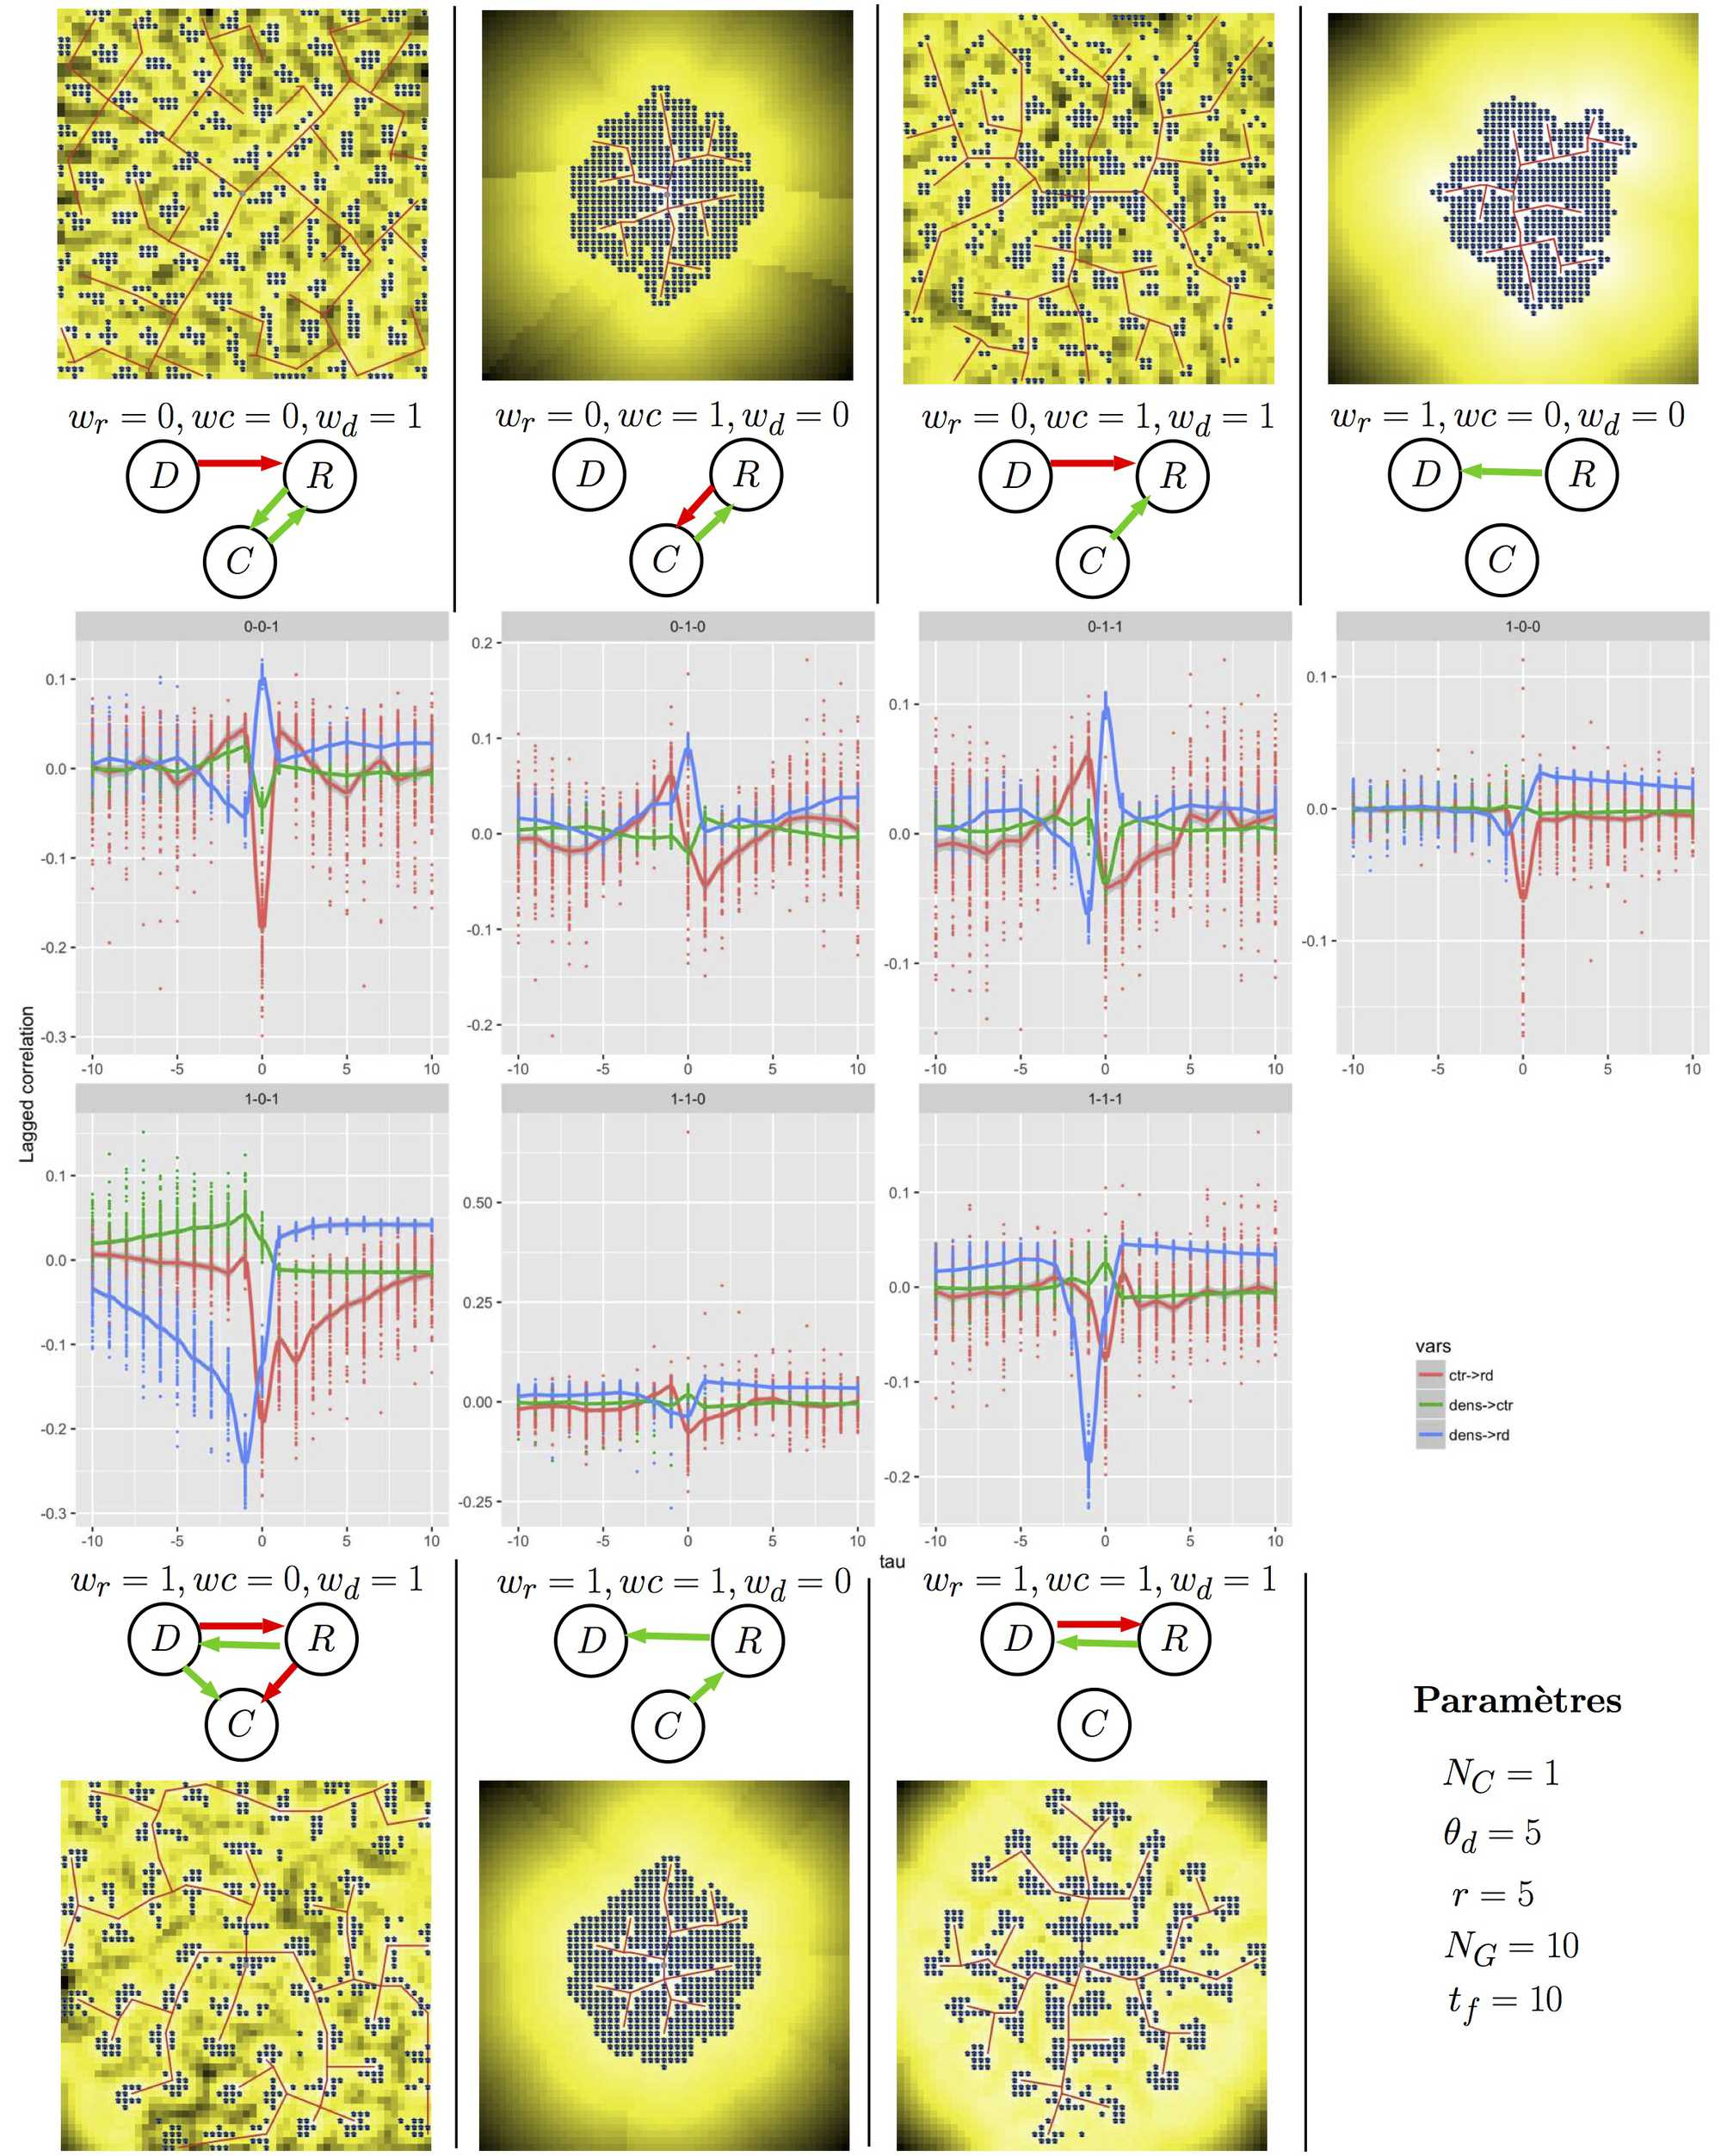
\includegraphics[height=0.9\textheight]{figures/rbd_4-2-2-fig-causalityregimes-exrdb.jpg}

%\column{0.35\textwidth}
%\justify
%\textit{Profiles of lagged correlations unveil diverse interaction networks between variables : towards a definition of causality regimes, including co-evolution in some cases.}


%\end{columns}
%
%}






\sframe{A Morphogenesis Model of co-evolution}{

\justify

\vspace{-1cm}

$\rightarrow$ Coupled grid population distribution and vector transportation network, following the core of \cite{raimbault2014hybrid}

\medskip

$\rightarrow$ Local morphological and functional variables determine a patch-value, driving new population attribution through preferential attachment ; combined to population diffusion (reaction-diffusion processes studied before)

% Comment Arnaud : réaction-diffusion ?

\medskip

$\rightarrow$ Network growth is also driven by morphological, functional and local network measures, following diverse heuristics corresponding to different processes (multi-modeling)

\bigskip
\bigskip

\textit{Local variables and network properties induce feedback on both, thus a strong coupling capturing the \textbf{co-evolution}}

}



\sframe{Model : Specification}{

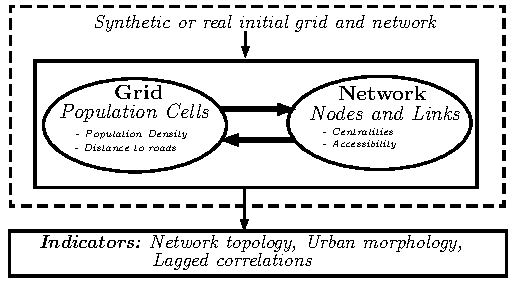
\includegraphics[width=\textwidth]{figures/coevol_mesocoevol}

}



\sframe{Network Generation: multi-modeling network growth}{

At fixed time steps :

\begin{enumerate}
	\item Add new nodes preferentially to new population and connect them
	\item \justify Variable heuristic for new links, among: nothing, random, gravity-based deterministic breakdown, gravity-based random breakdown (from \cite{schmitt2014modelisation}), cost-benefits (from \cite{louf2013emergence}), biological network generation (based on \cite{tero2010rules})
\end{enumerate}

\medskip

\centering

\frame{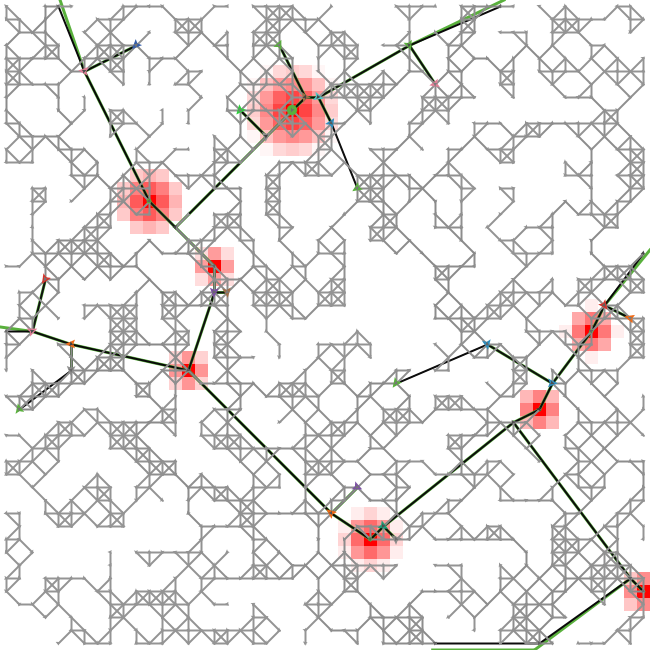
\includegraphics[height=0.31\textwidth]{figures/coevol_example-bio-process-1}}\hspace{0.2cm}
\frame{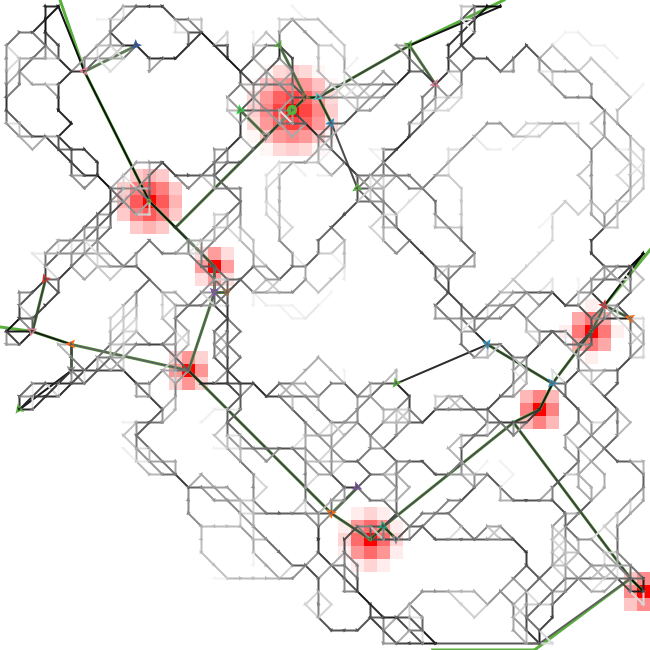
\includegraphics[height=0.31\textwidth]{figures/coevol_example-bio-process-1-tick80}}

\footnotesize

\textit{Intermediate stage for biological network generation}

}



\sframe{Generated Urban Shapes: Network}{


\centering

%\frame{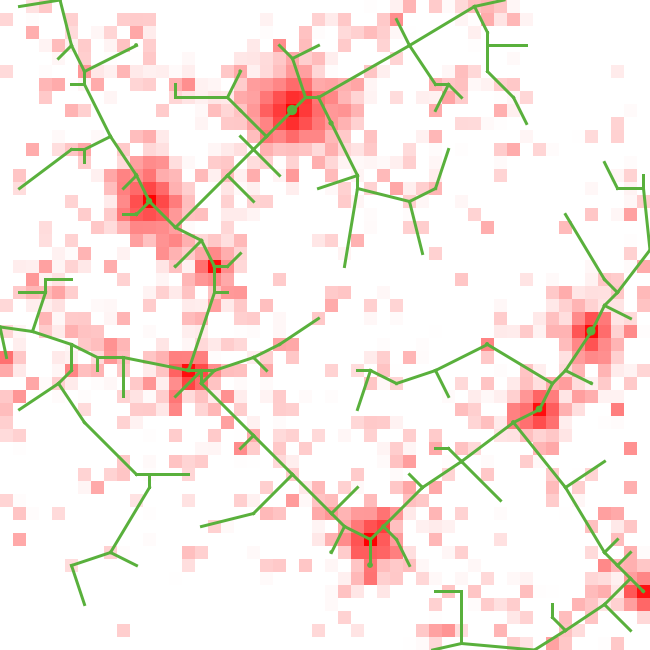
\includegraphics[width=0.28\textwidth]{figures/coevol_example_nw-connection}}\hspace{0.1cm}
%\frame{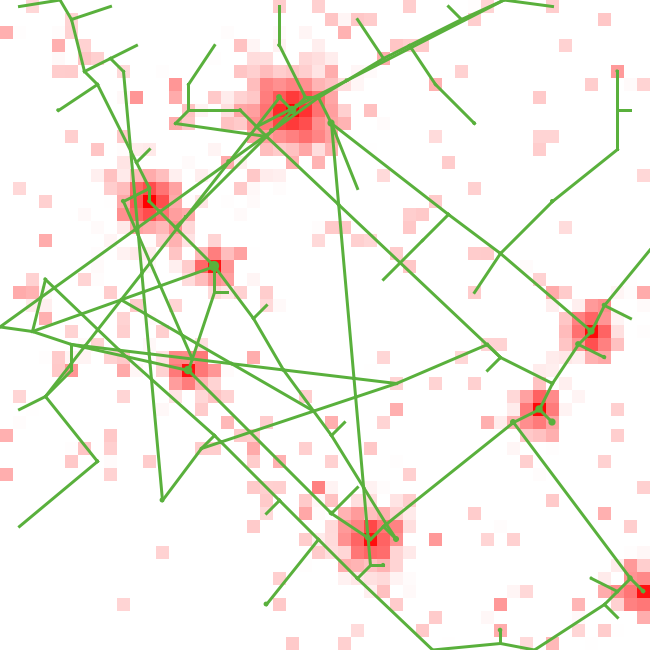
\includegraphics[width=0.28\textwidth]{figures/coevol_example_nw-random}}\hspace{0.1cm}
%\frame{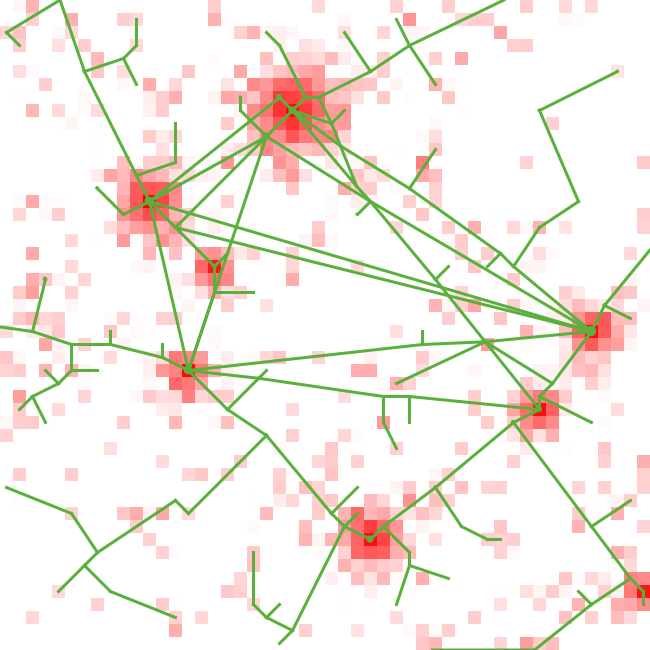
\includegraphics[width=0.28\textwidth]{figures/coevol_example_nw-gravity}}\\\vspace{0.1cm}
%\frame{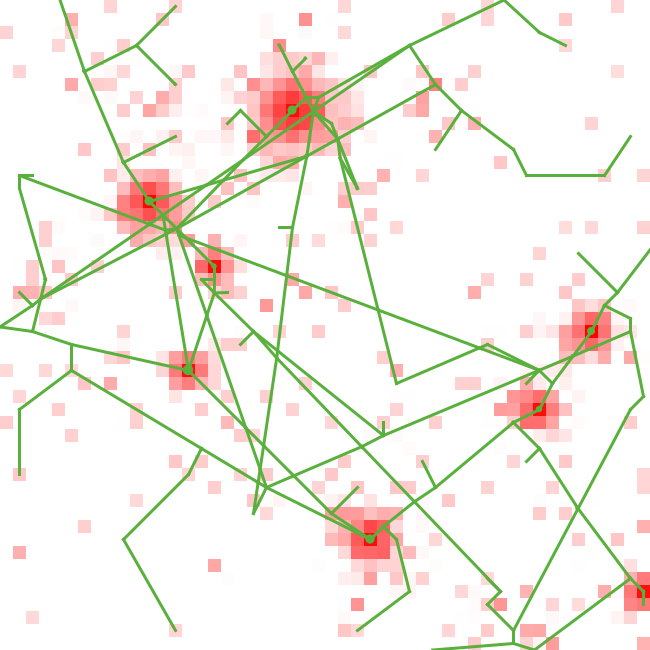
\includegraphics[width=0.28\textwidth]{figures/coevol_example_nw-rndbrkdwn}}\hspace{0.1cm}
%\frame{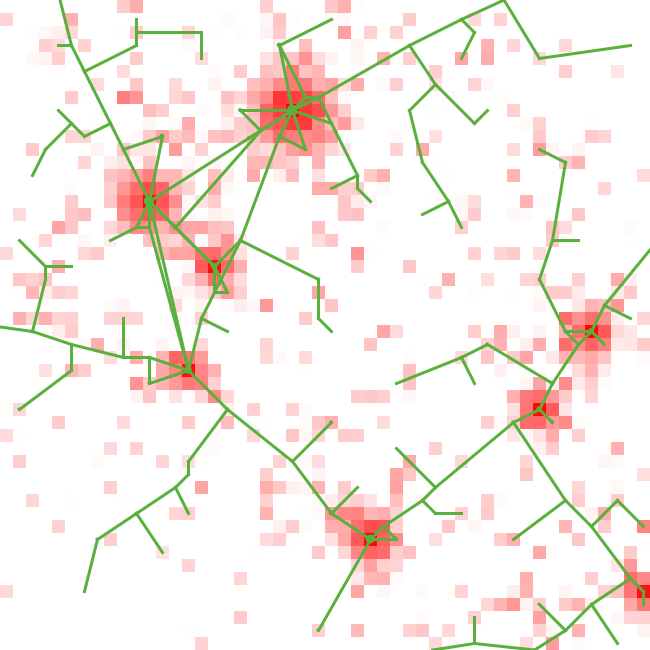
\includegraphics[width=0.28\textwidth]{figures/coevol_example_nw-cost}}\hspace{0.1cm}
%\frame{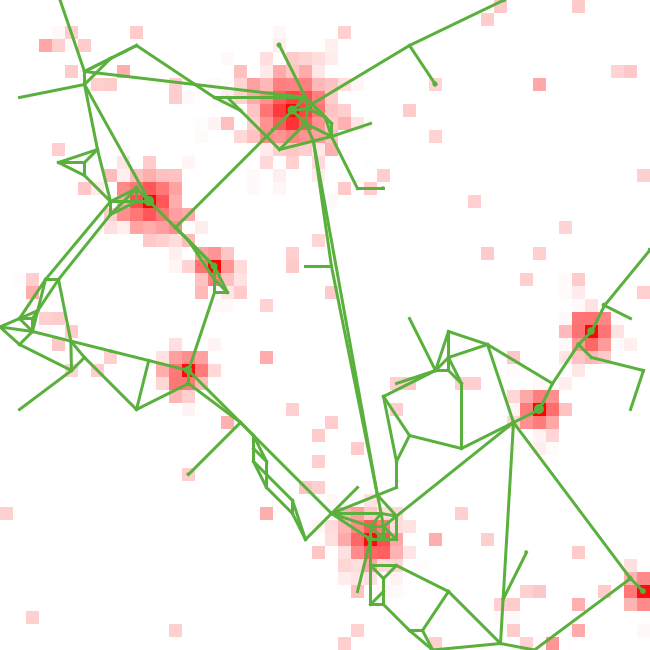
\includegraphics[width=0.28\textwidth]{figures/coevol_example_nw-bio}}

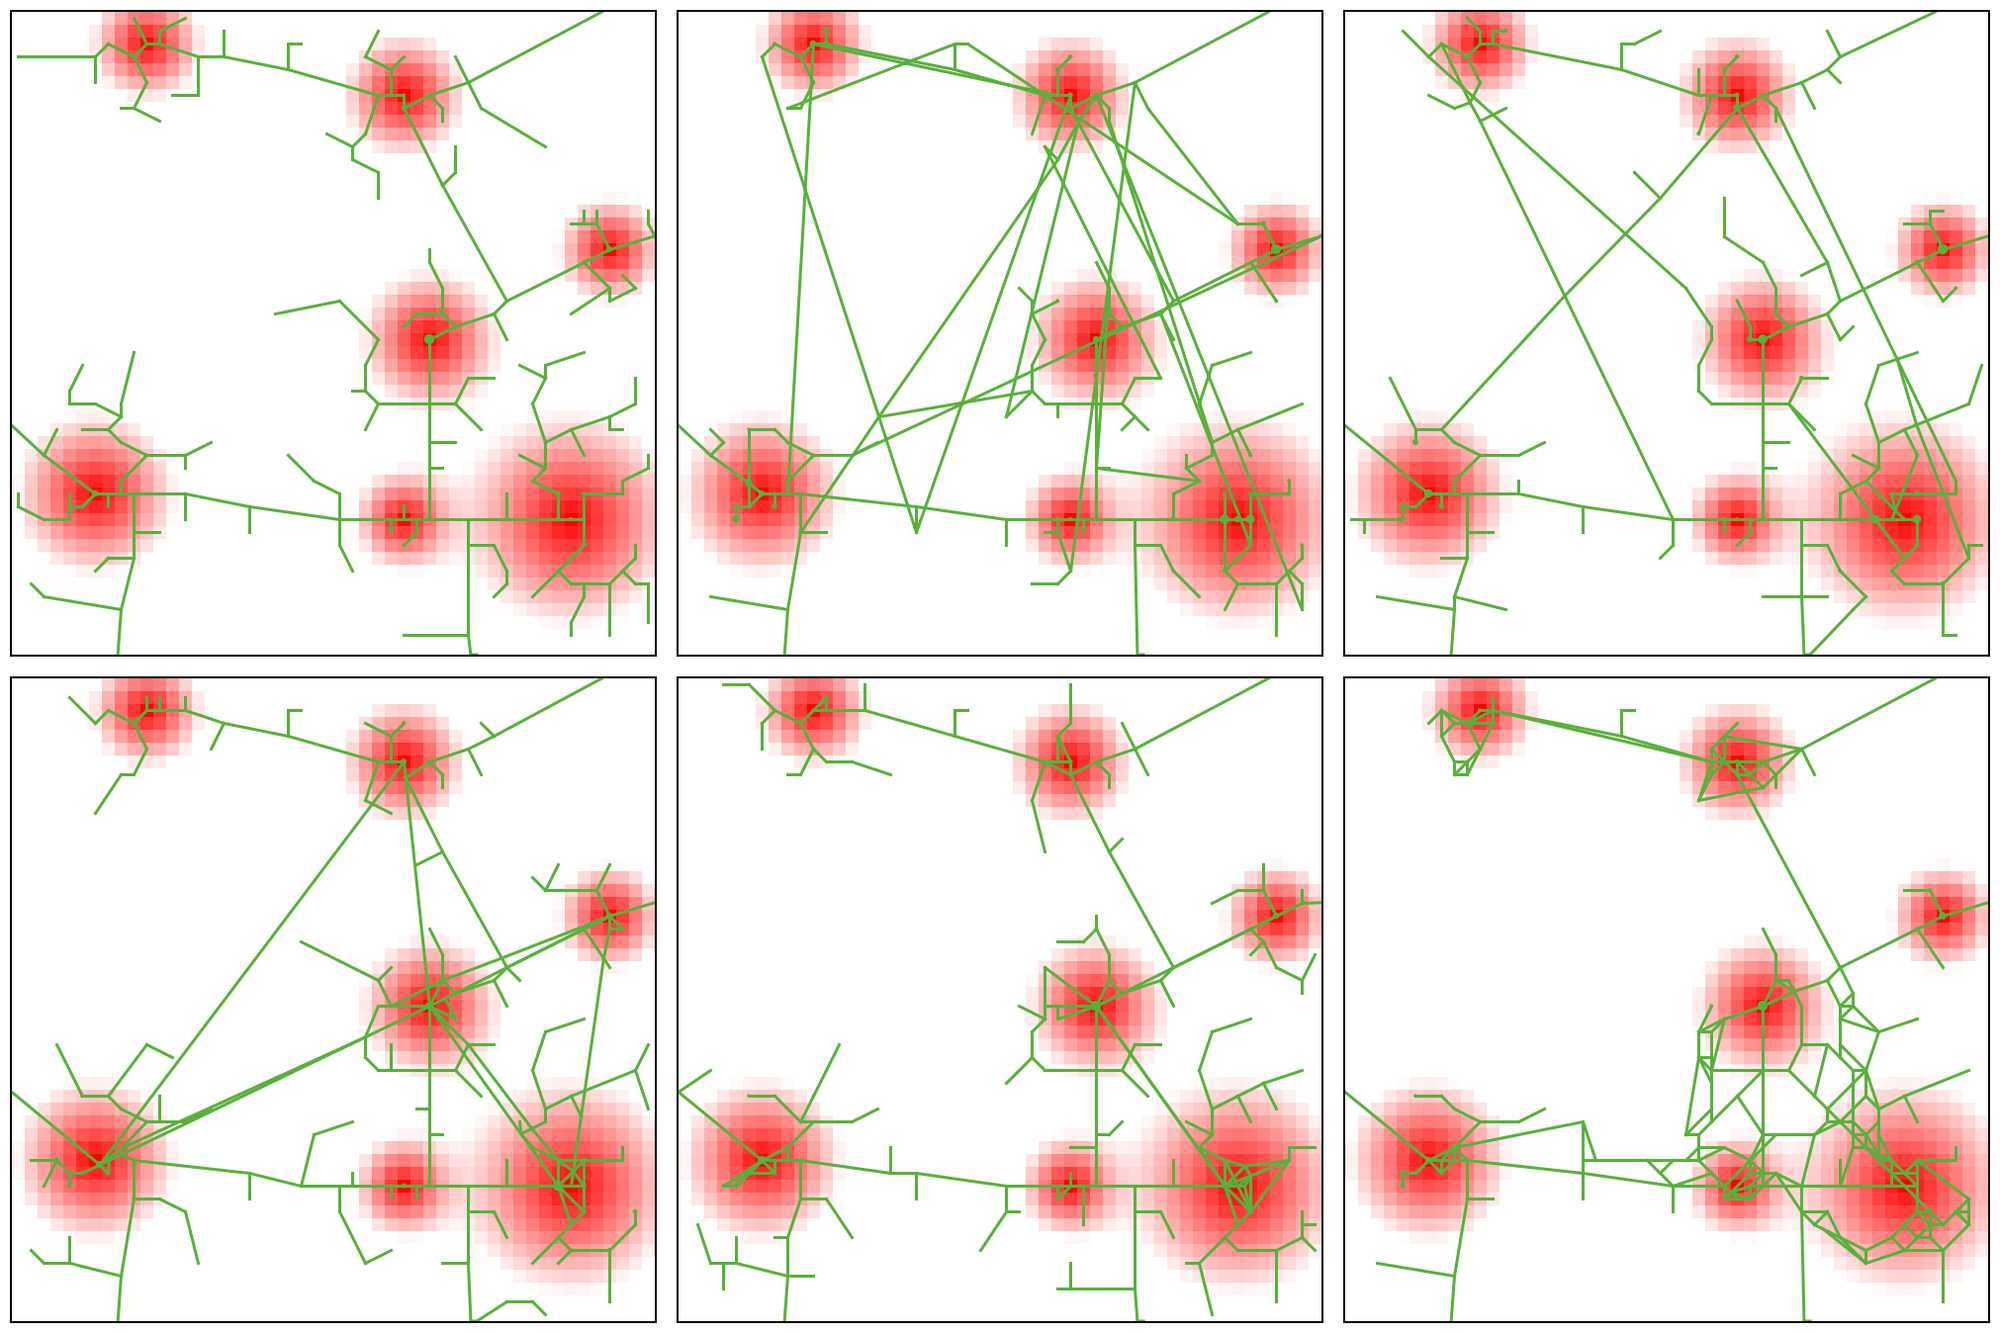
\includegraphics[width=\textwidth]{figures/7-1-2-fig-networkgrowth-examples.jpg}

\footnotesize\textit{In order: connection; random; deterministic breakdown; random breakdown; cost-driven; biological.}

}


\sframe{Results : Feasible space of network topologies}{

\centering

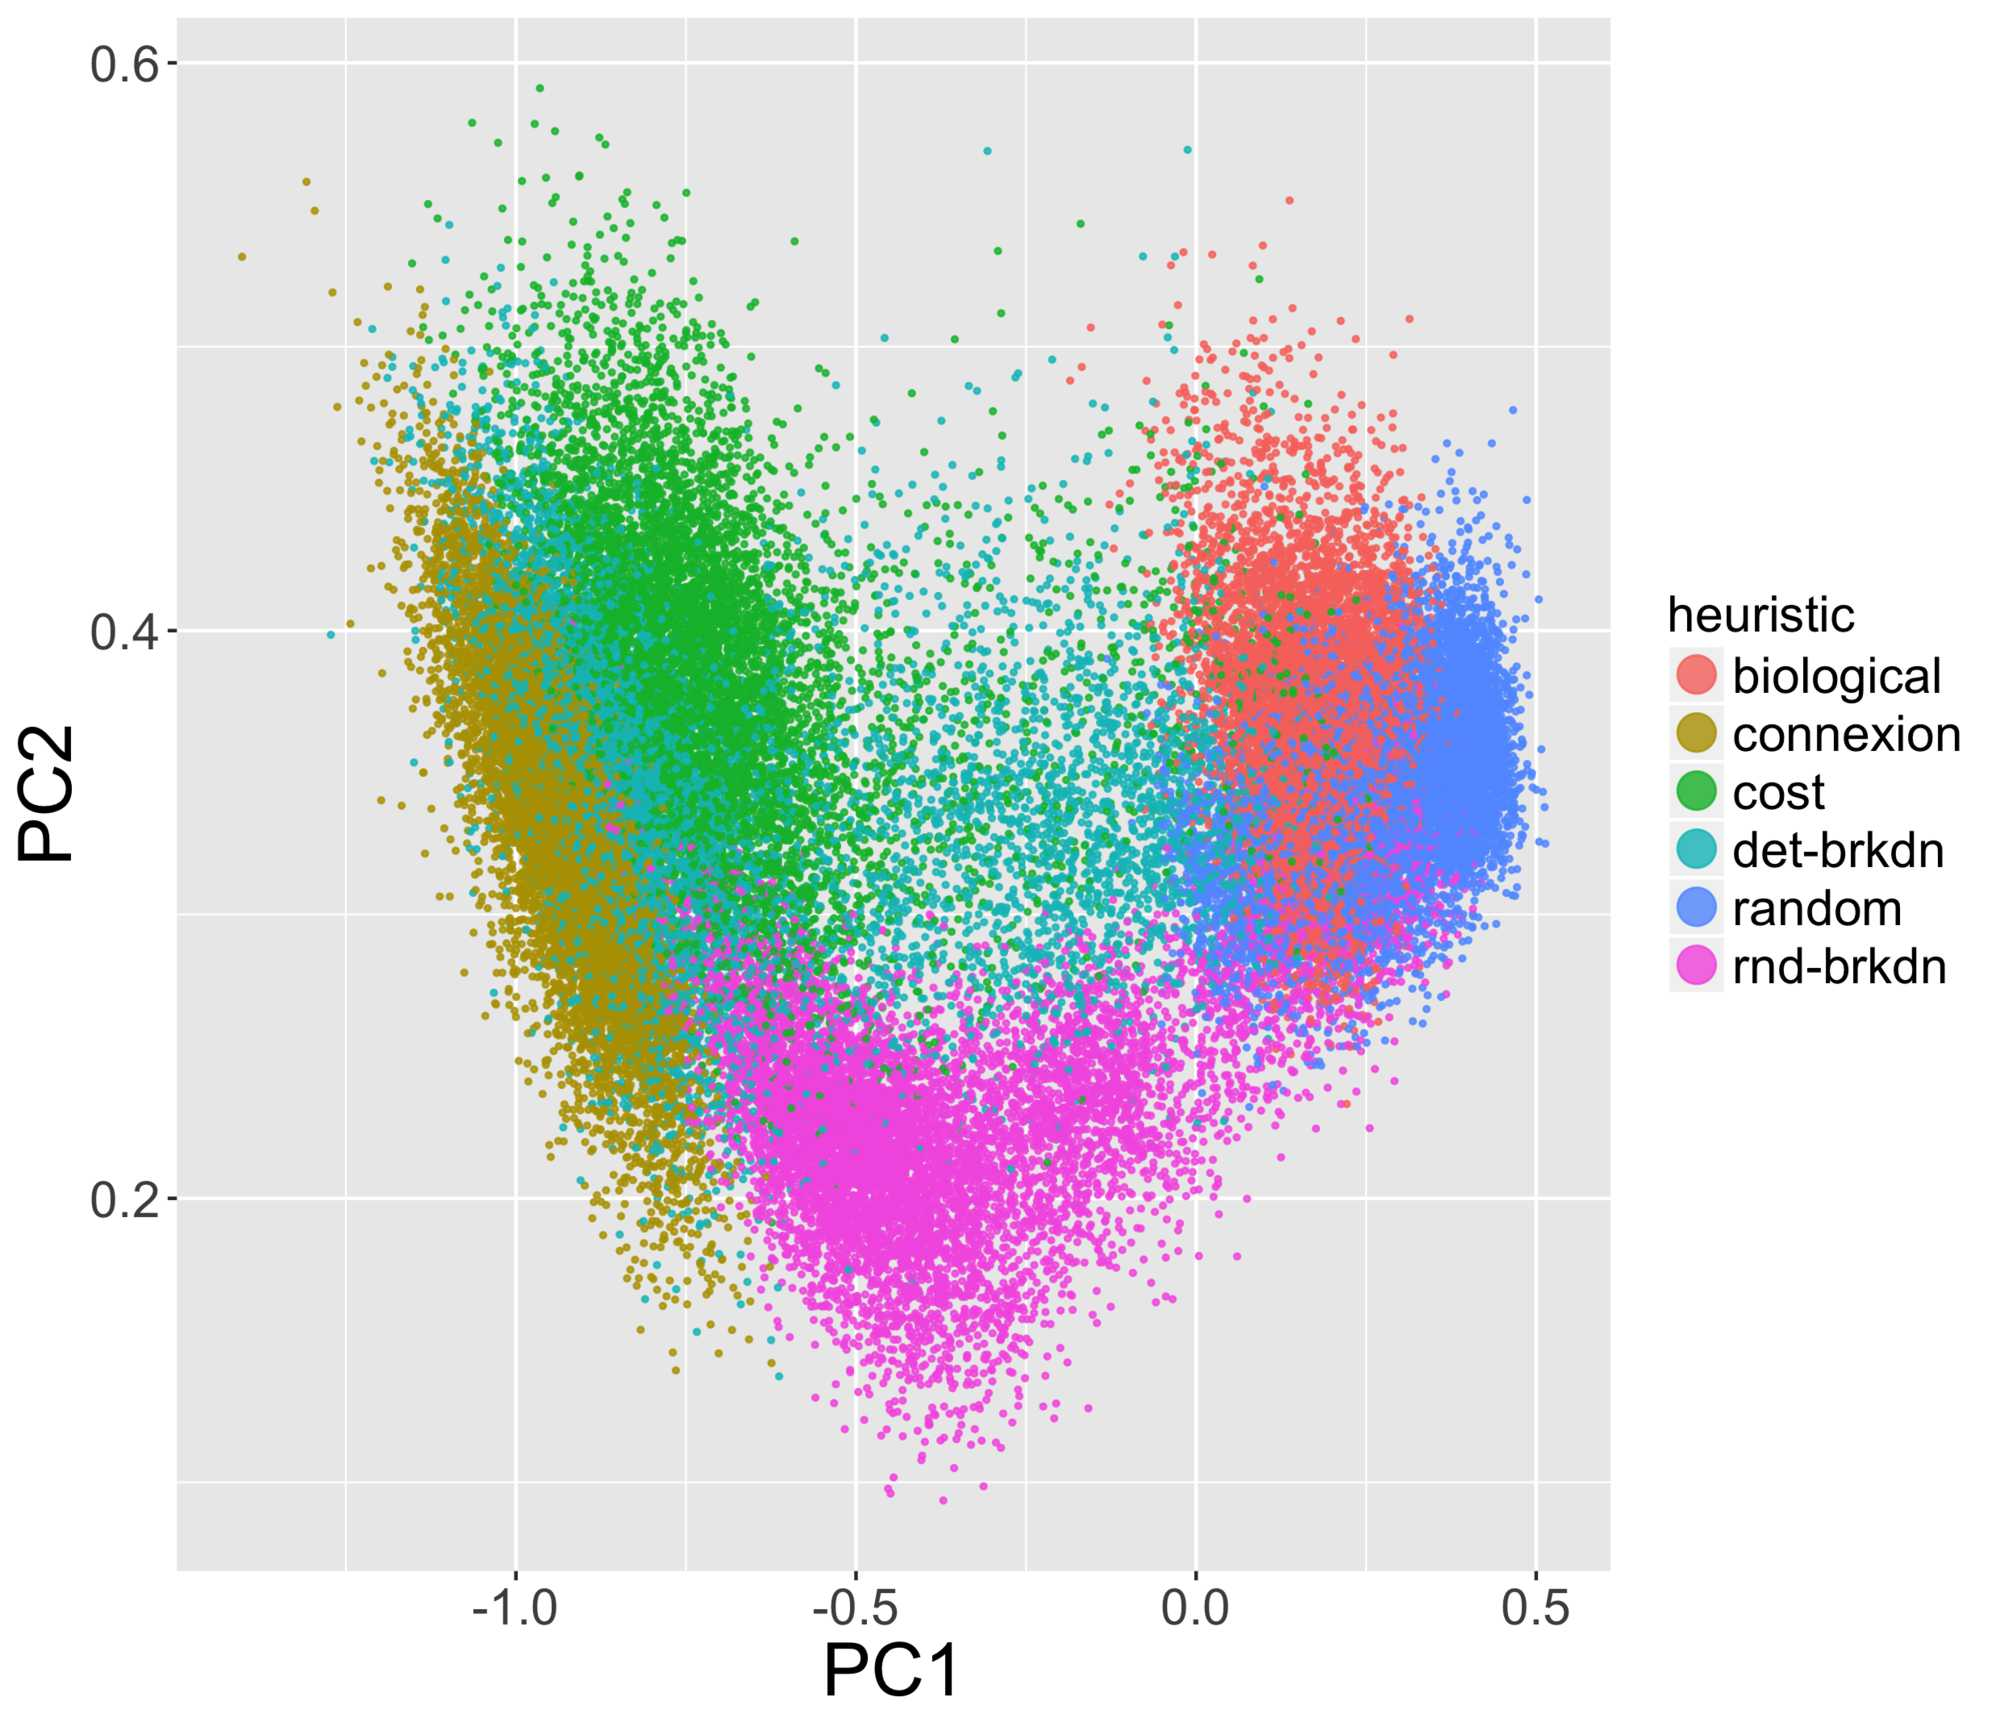
\includegraphics[height=0.8\textheight]{figures/7-1-2-fig-networkgrowth-feasiblespace.jpg}

}




\sframe{Results : Network Heuristics}{

\justify

\textit{Comparison of feasible space for network indicators with fixed density}

\bigskip

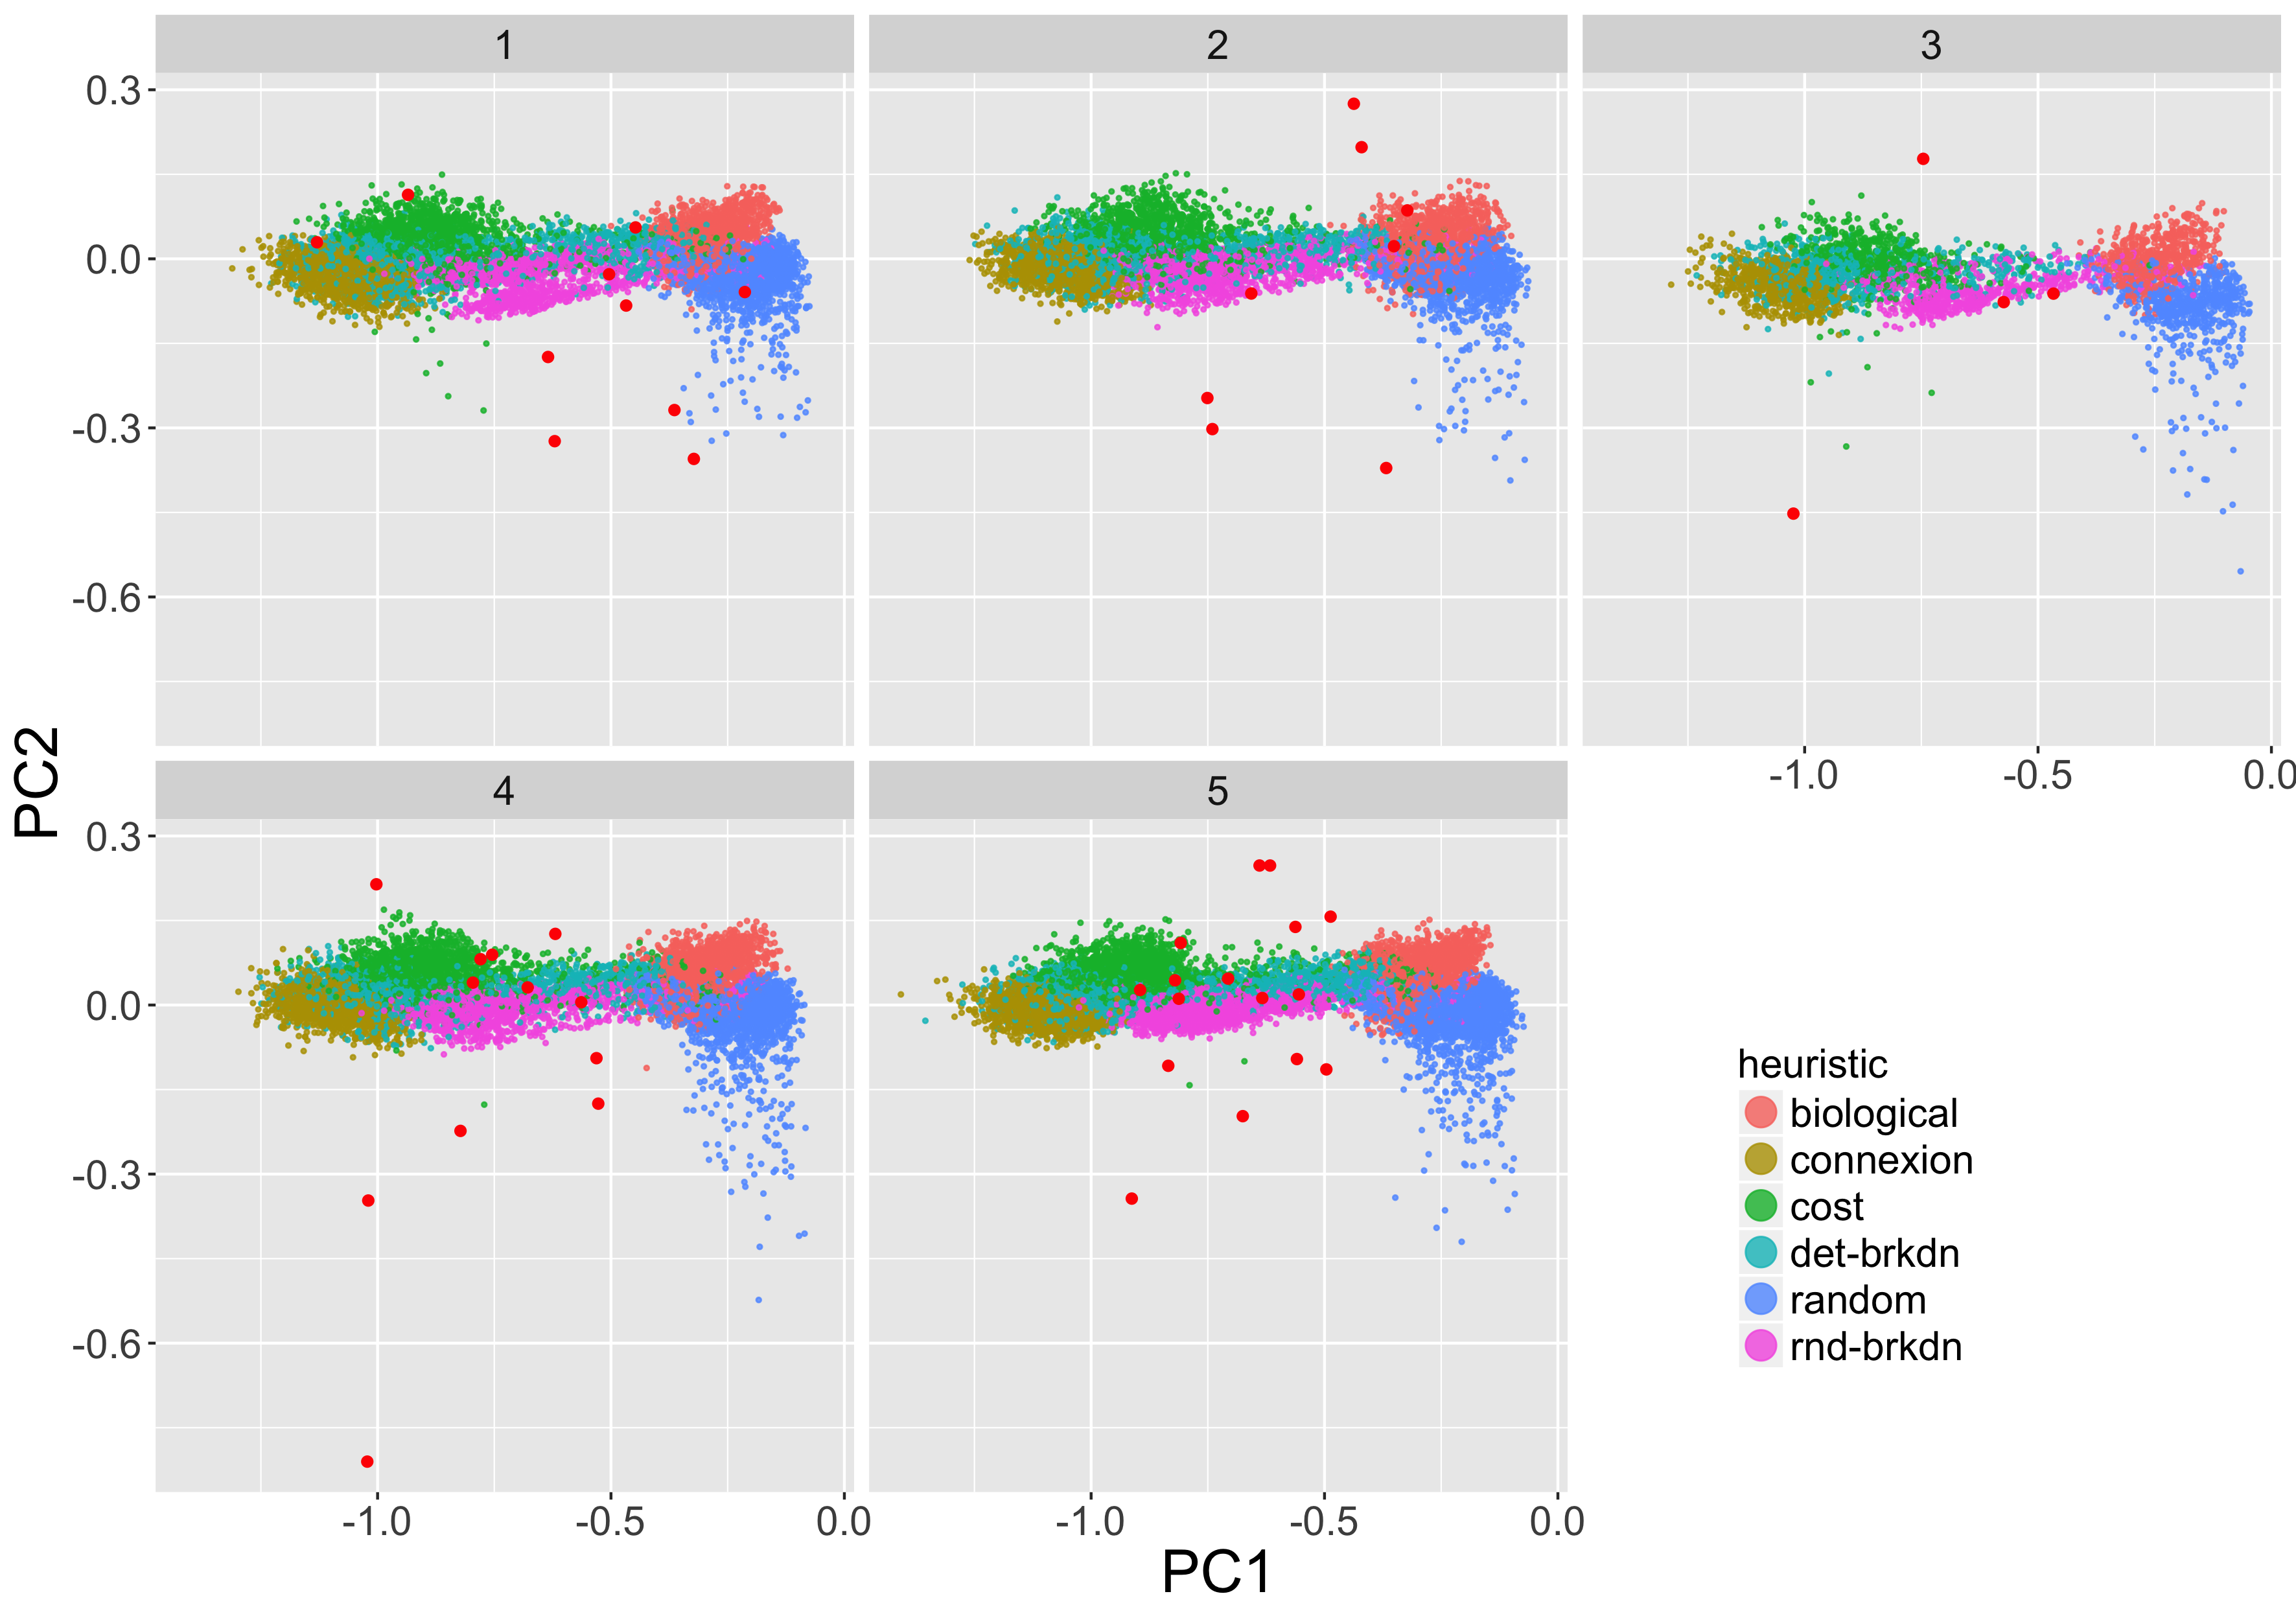
\includegraphics[width=0.52\textwidth,height=0.6\textheight]{figures/coevol_feasible_space_withreal_pca_bymorph}
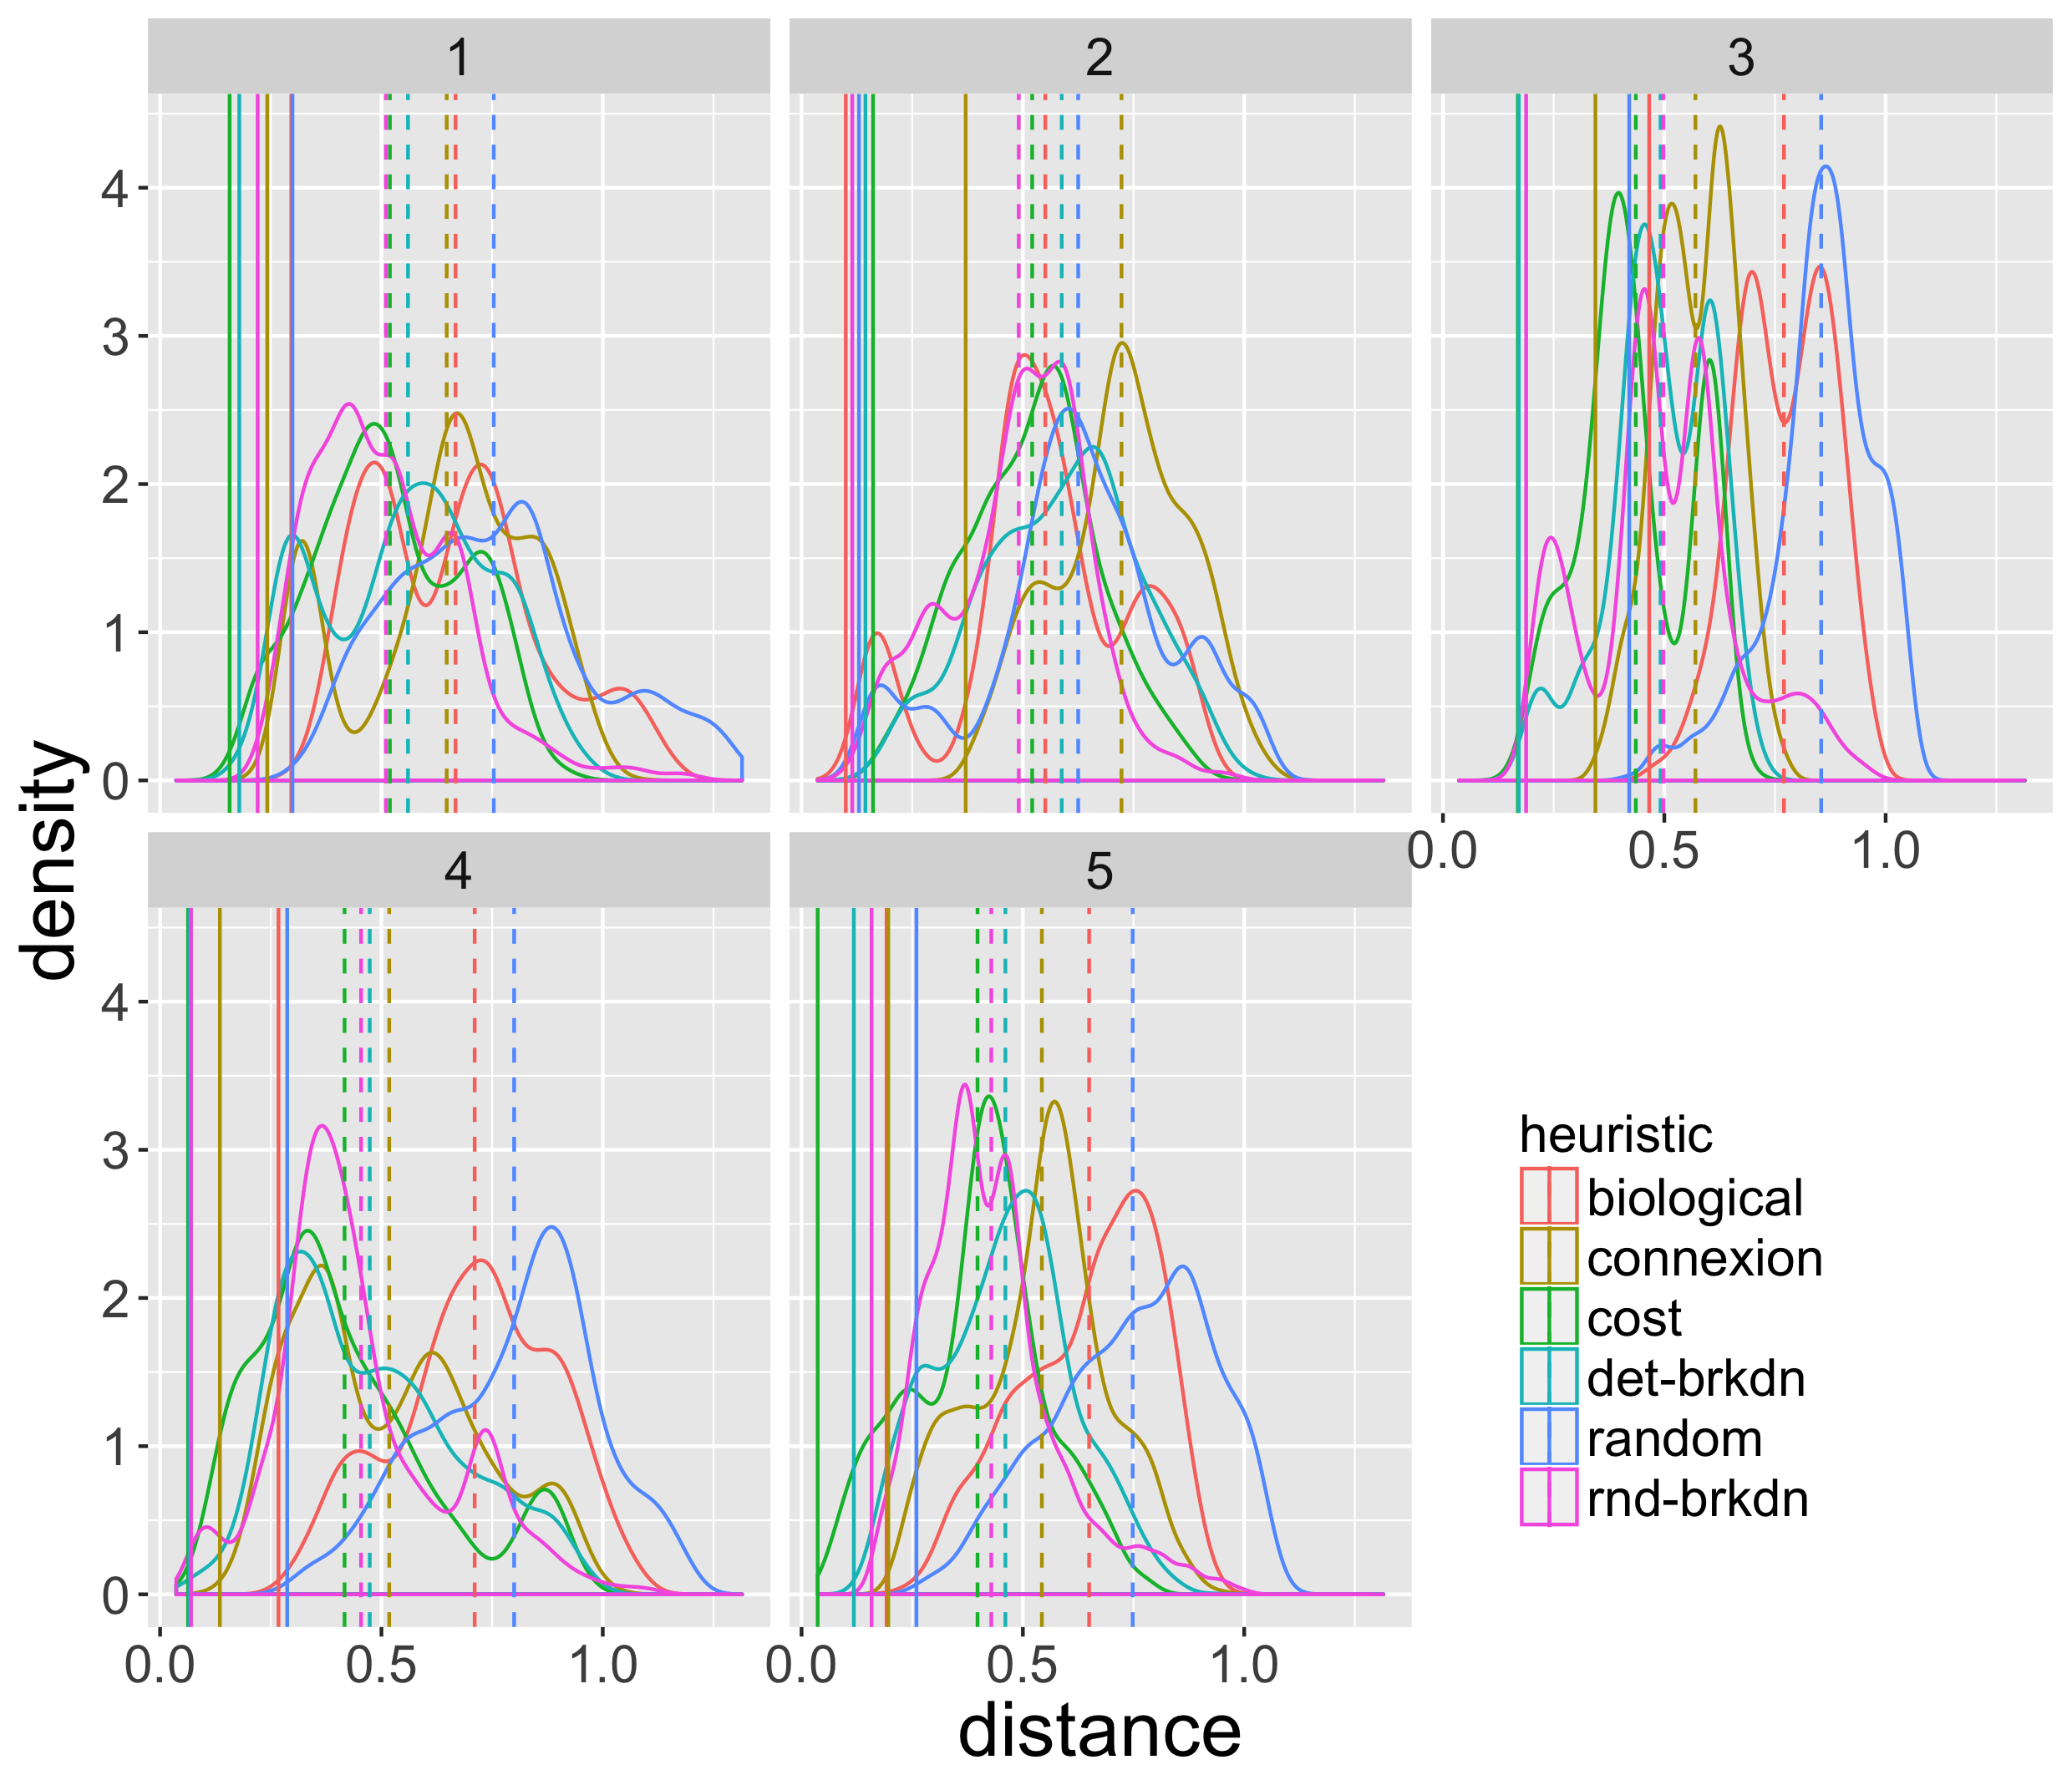
\includegraphics[width=0.43\textwidth,height=0.6\textheight]{figures/coevol_distance_real_bymorph}

\footnotesize

\textit{(Left) Feasible spaces by morphological class and network heuristic; (Right) Distribution of distances to topologies of real networks}

}






\sframe{Generated Urban Shapes: Urban Form}{

\centering

\frame{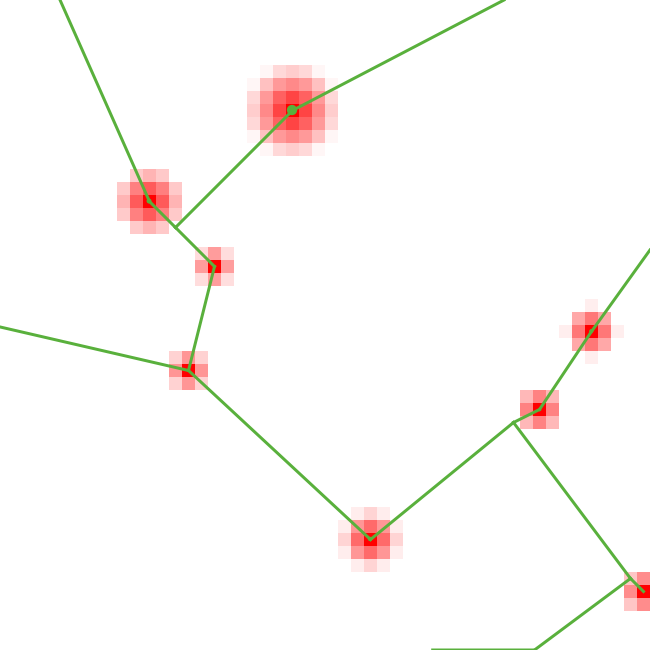
\includegraphics[width=0.28\textwidth]{figures/coevol_example_synthsetup}}\hspace{0.1cm}
\frame{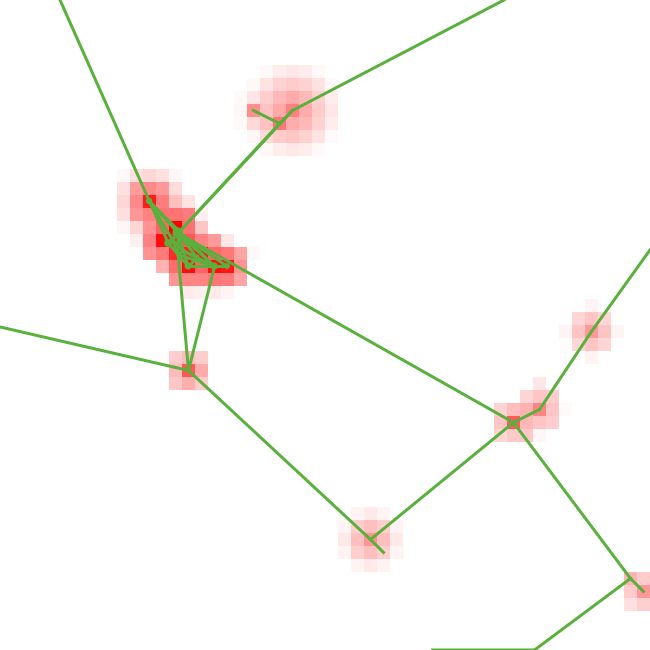
\includegraphics[width=0.28\textwidth]{figures/coevol_example_form-accessonly}}\hspace{0.1cm}
\frame{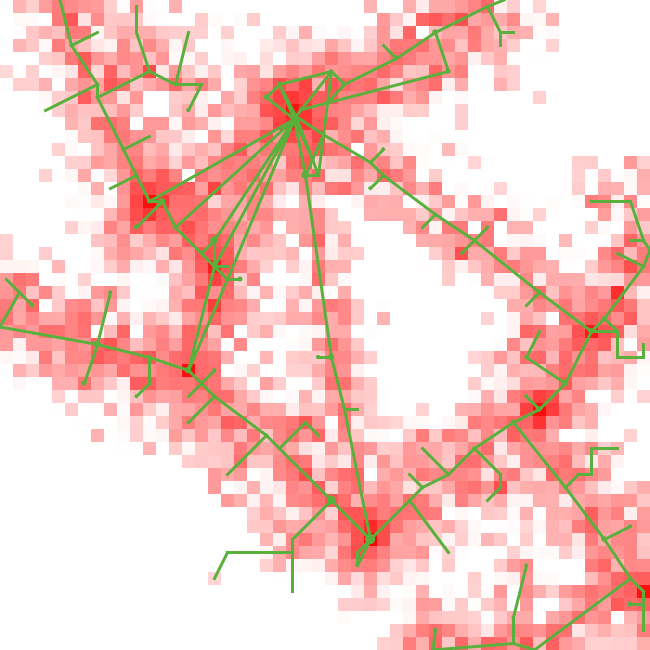
\includegraphics[width=0.28\textwidth]{figures/coevol_example_form-droadonly}}\\\vspace{0.1cm}
\frame{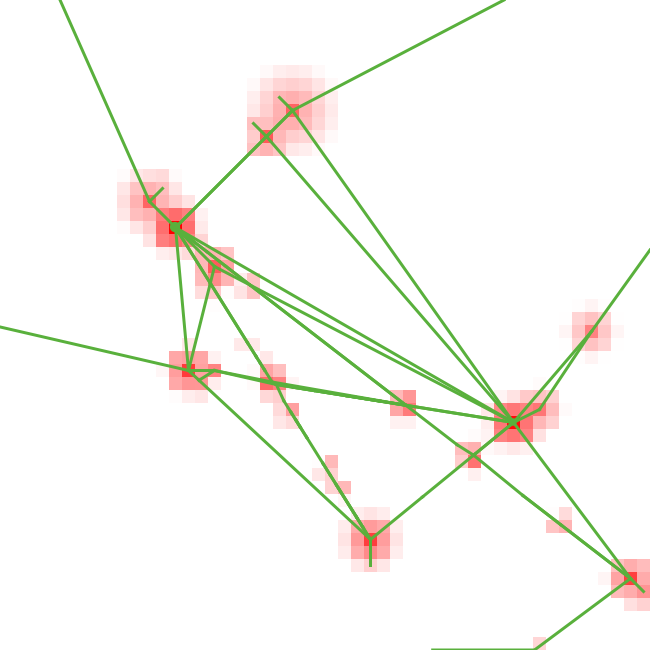
\includegraphics[width=0.28\textwidth]{figures/coevol_example_form-bwonly}}\hspace{0.1cm}
\frame{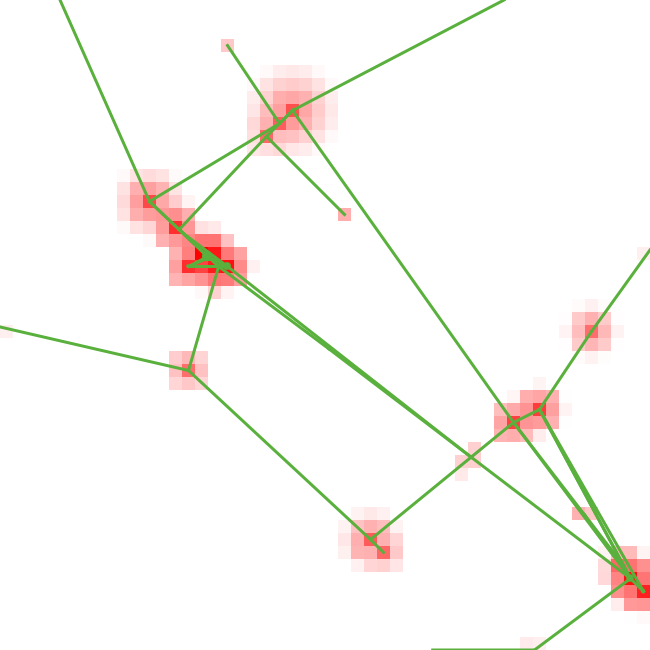
\includegraphics[width=0.28\textwidth]{figures/coevol_example_form-closenessonly}}\hspace{0.1cm}
\frame{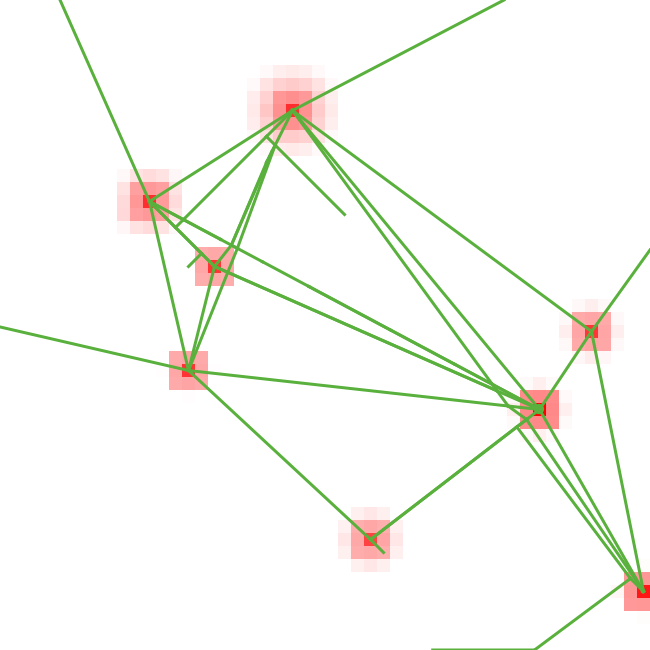
\includegraphics[width=0.28\textwidth]{figures/coevol_example_form-poponly}}

\footnotesize\textit{In order: setup; accessibility driven; road distance driven; betweenness driven; closeness driven; population driven.}

}











\sframe{Results : Calibration}{

\justify

\vspace{-0.5cm}

Calibration (model explored with OpenMole~\cite{reuillon2013openmole}, $\sim 10^6$ model runs) at the first order on morphological and topological objectives, and on correlations matrices.

\bigskip

\begin{columns}
\column{0.4\textwidth}
\centering
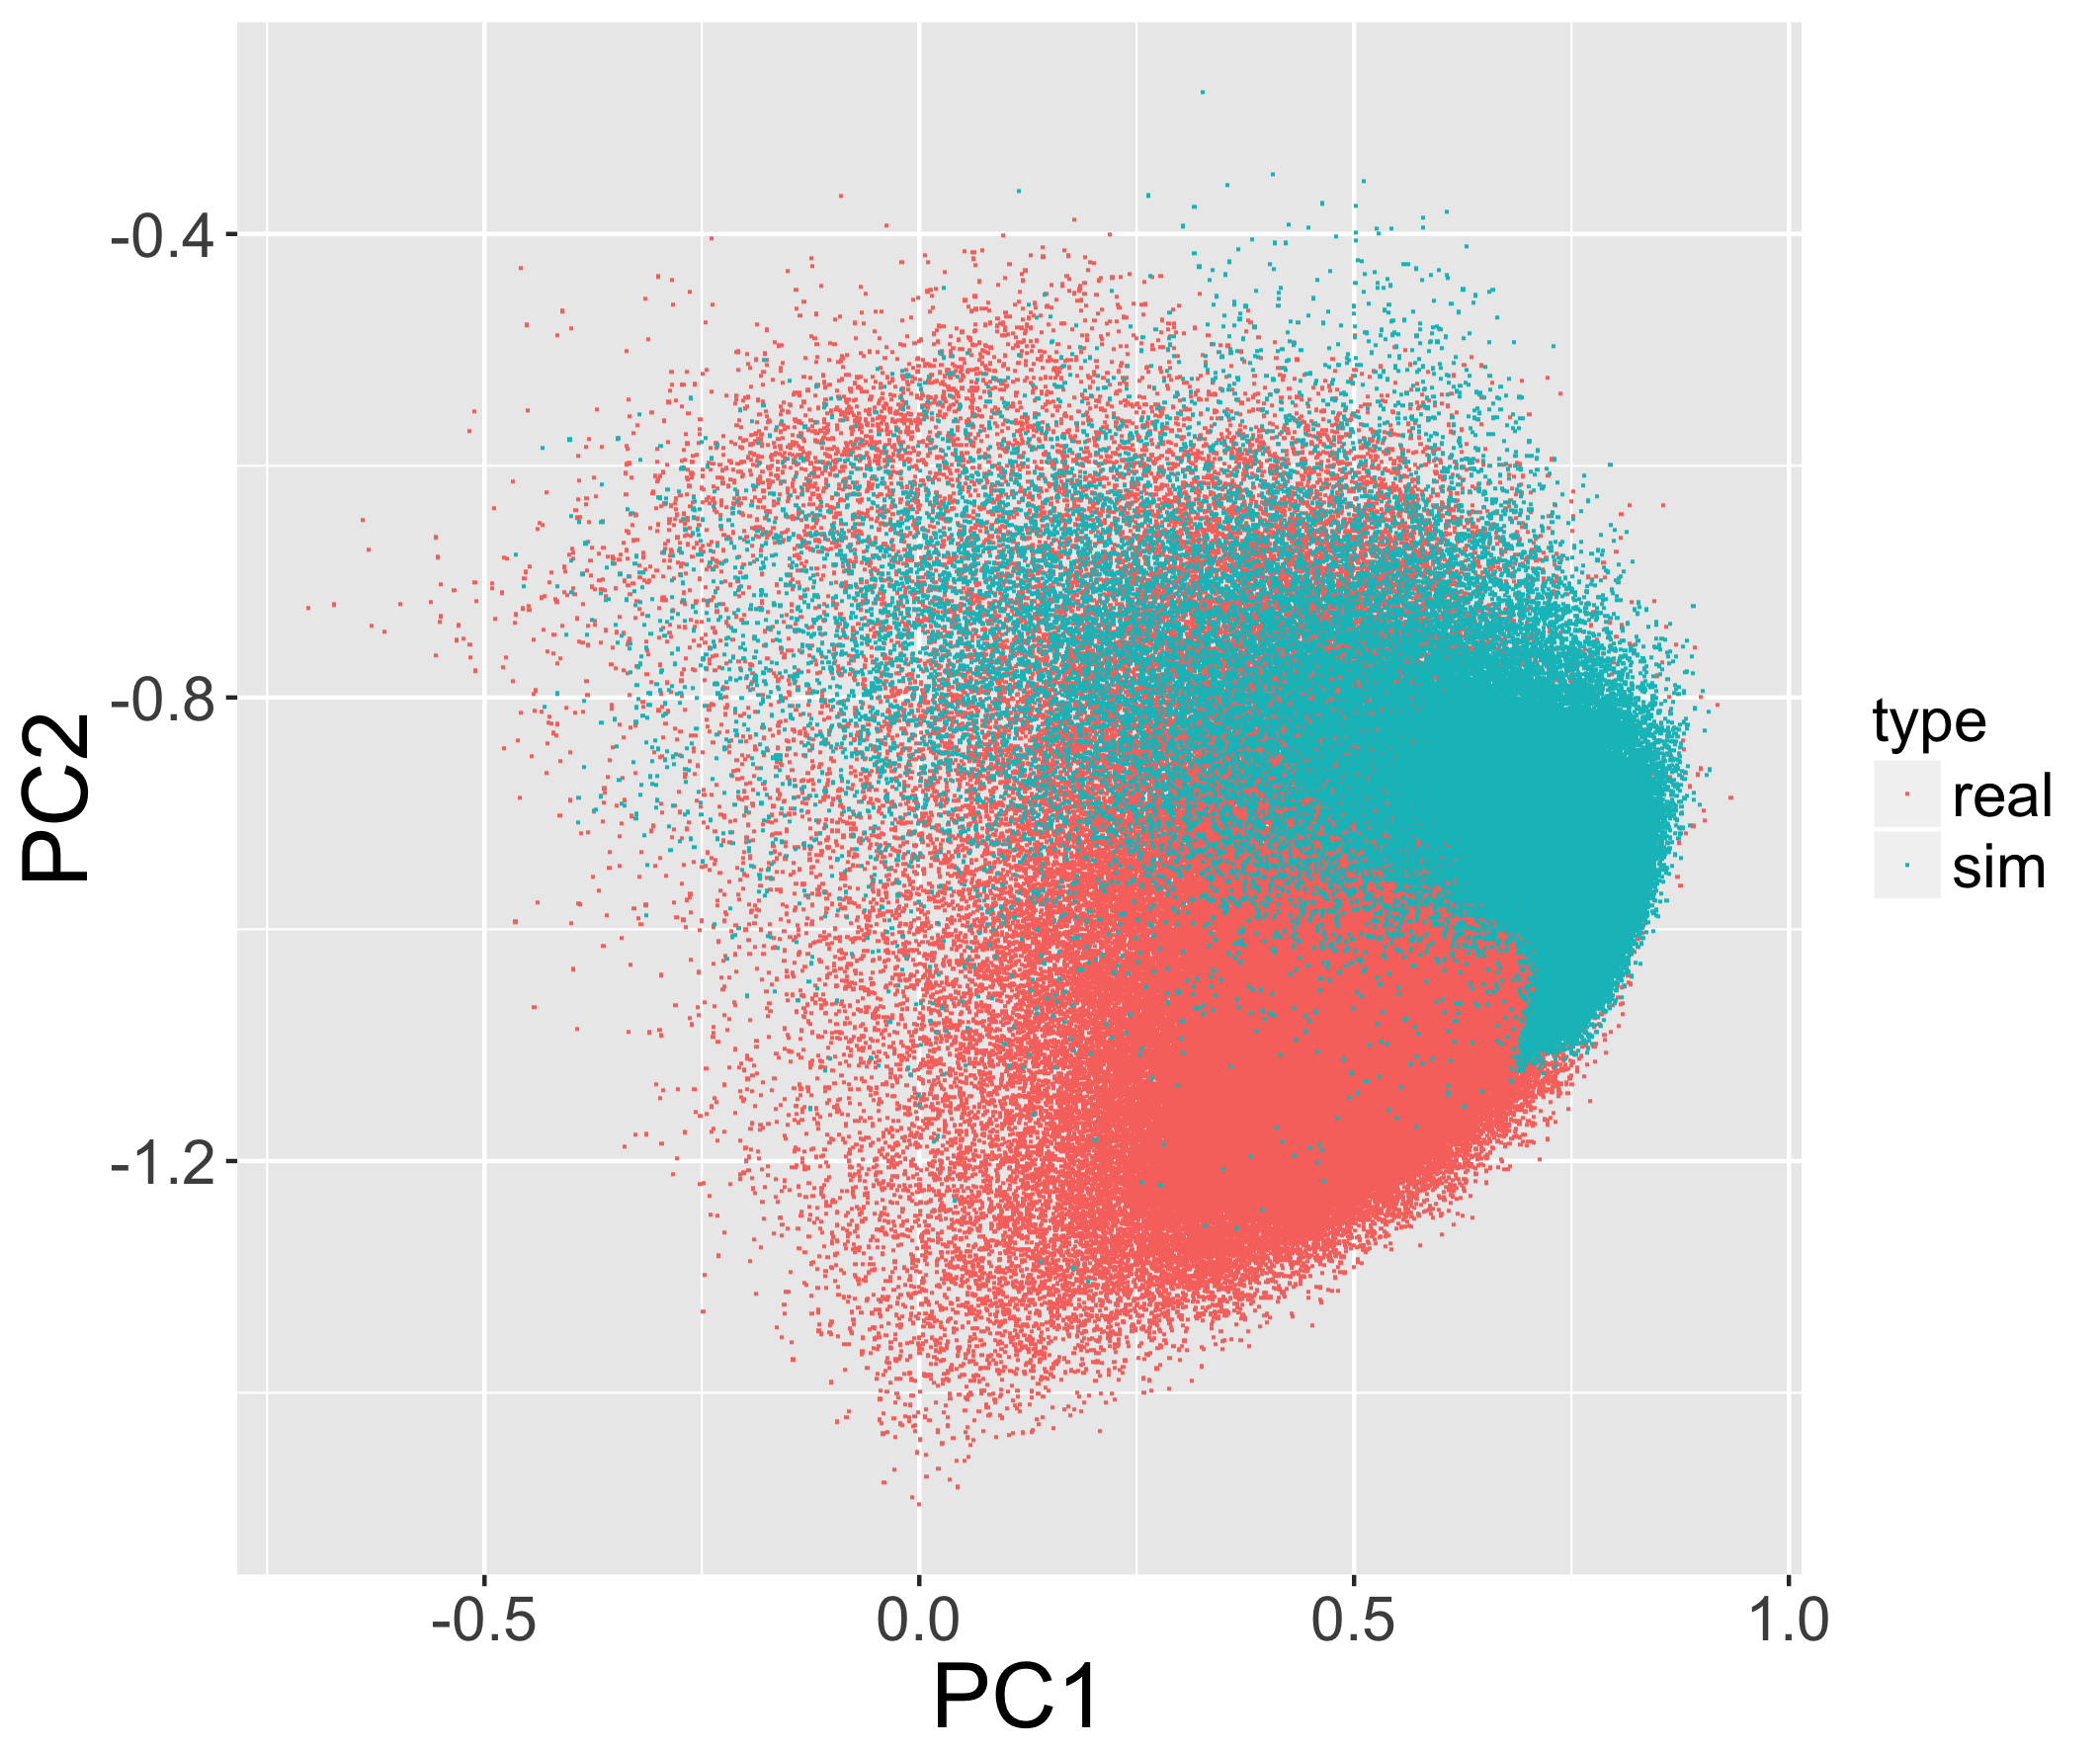
\includegraphics[width=\textwidth]{figures/coevol_pca_allobjs}
\column{0.2\textwidth}
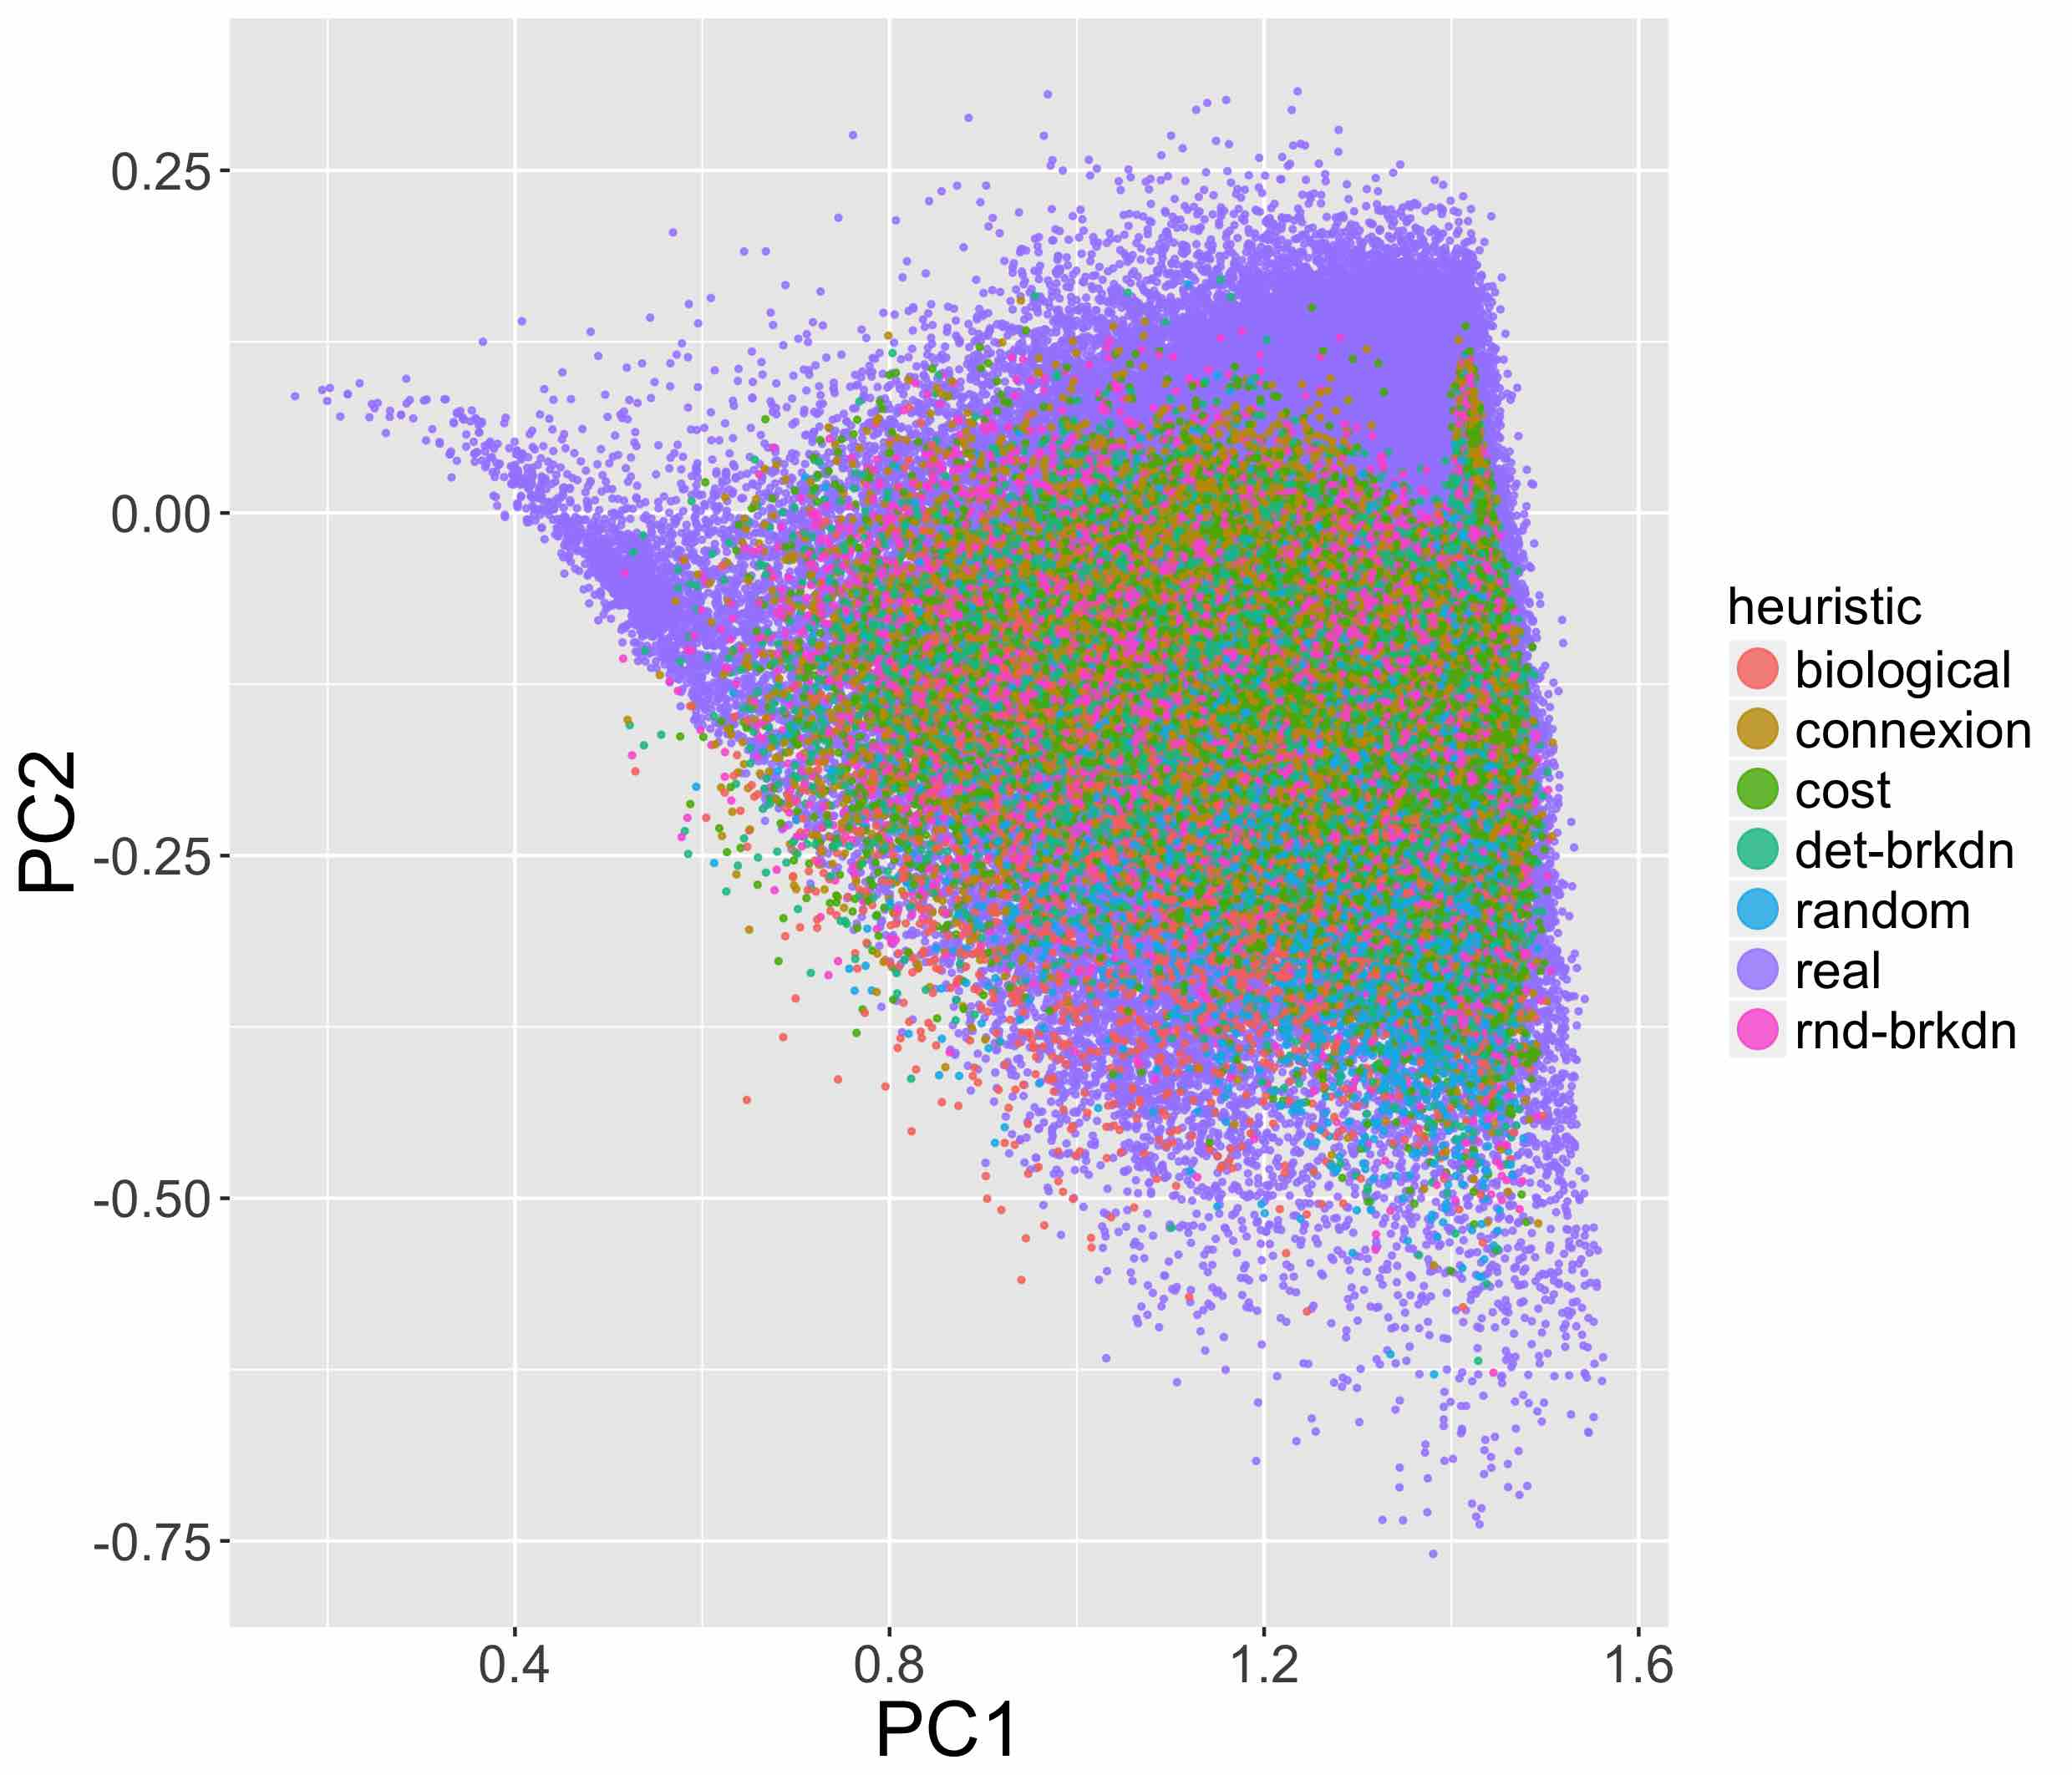
\includegraphics[width=\textwidth]{figures/coevol_pca_morpho_byheuristic}\\
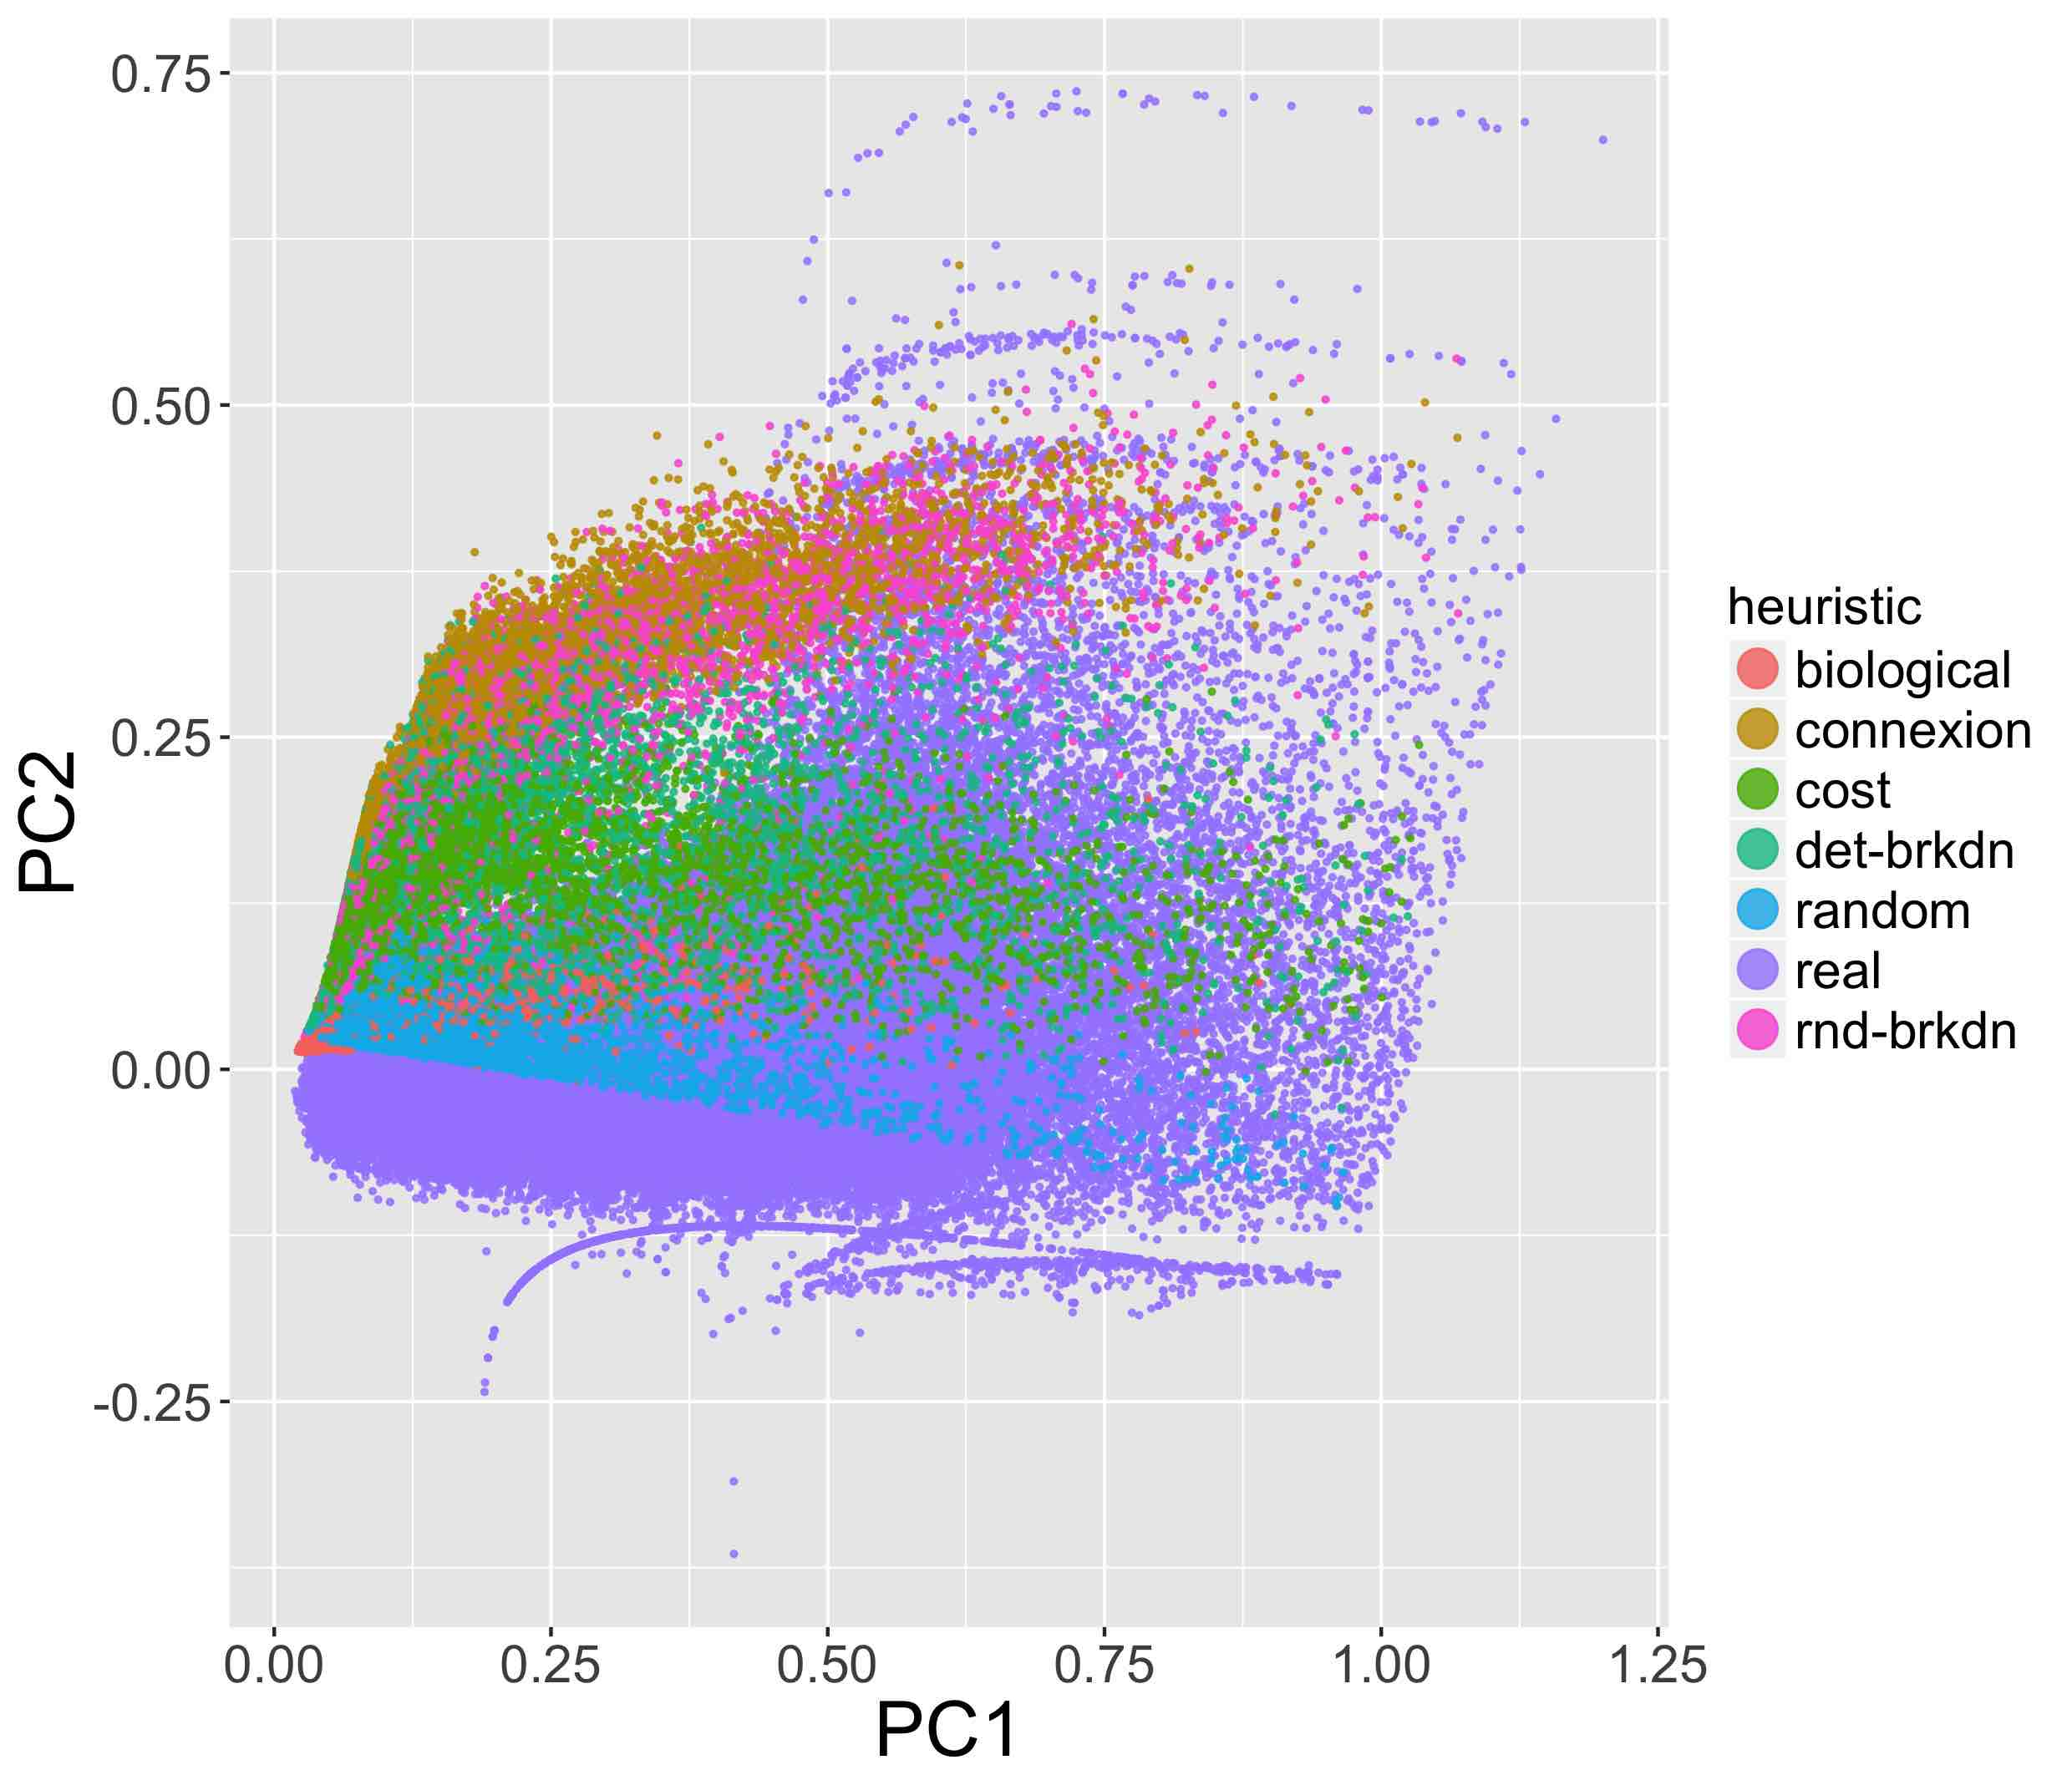
\includegraphics[width=\textwidth]{figures/coevol_pca_network_byheuristic}
\column{0.4\textwidth}
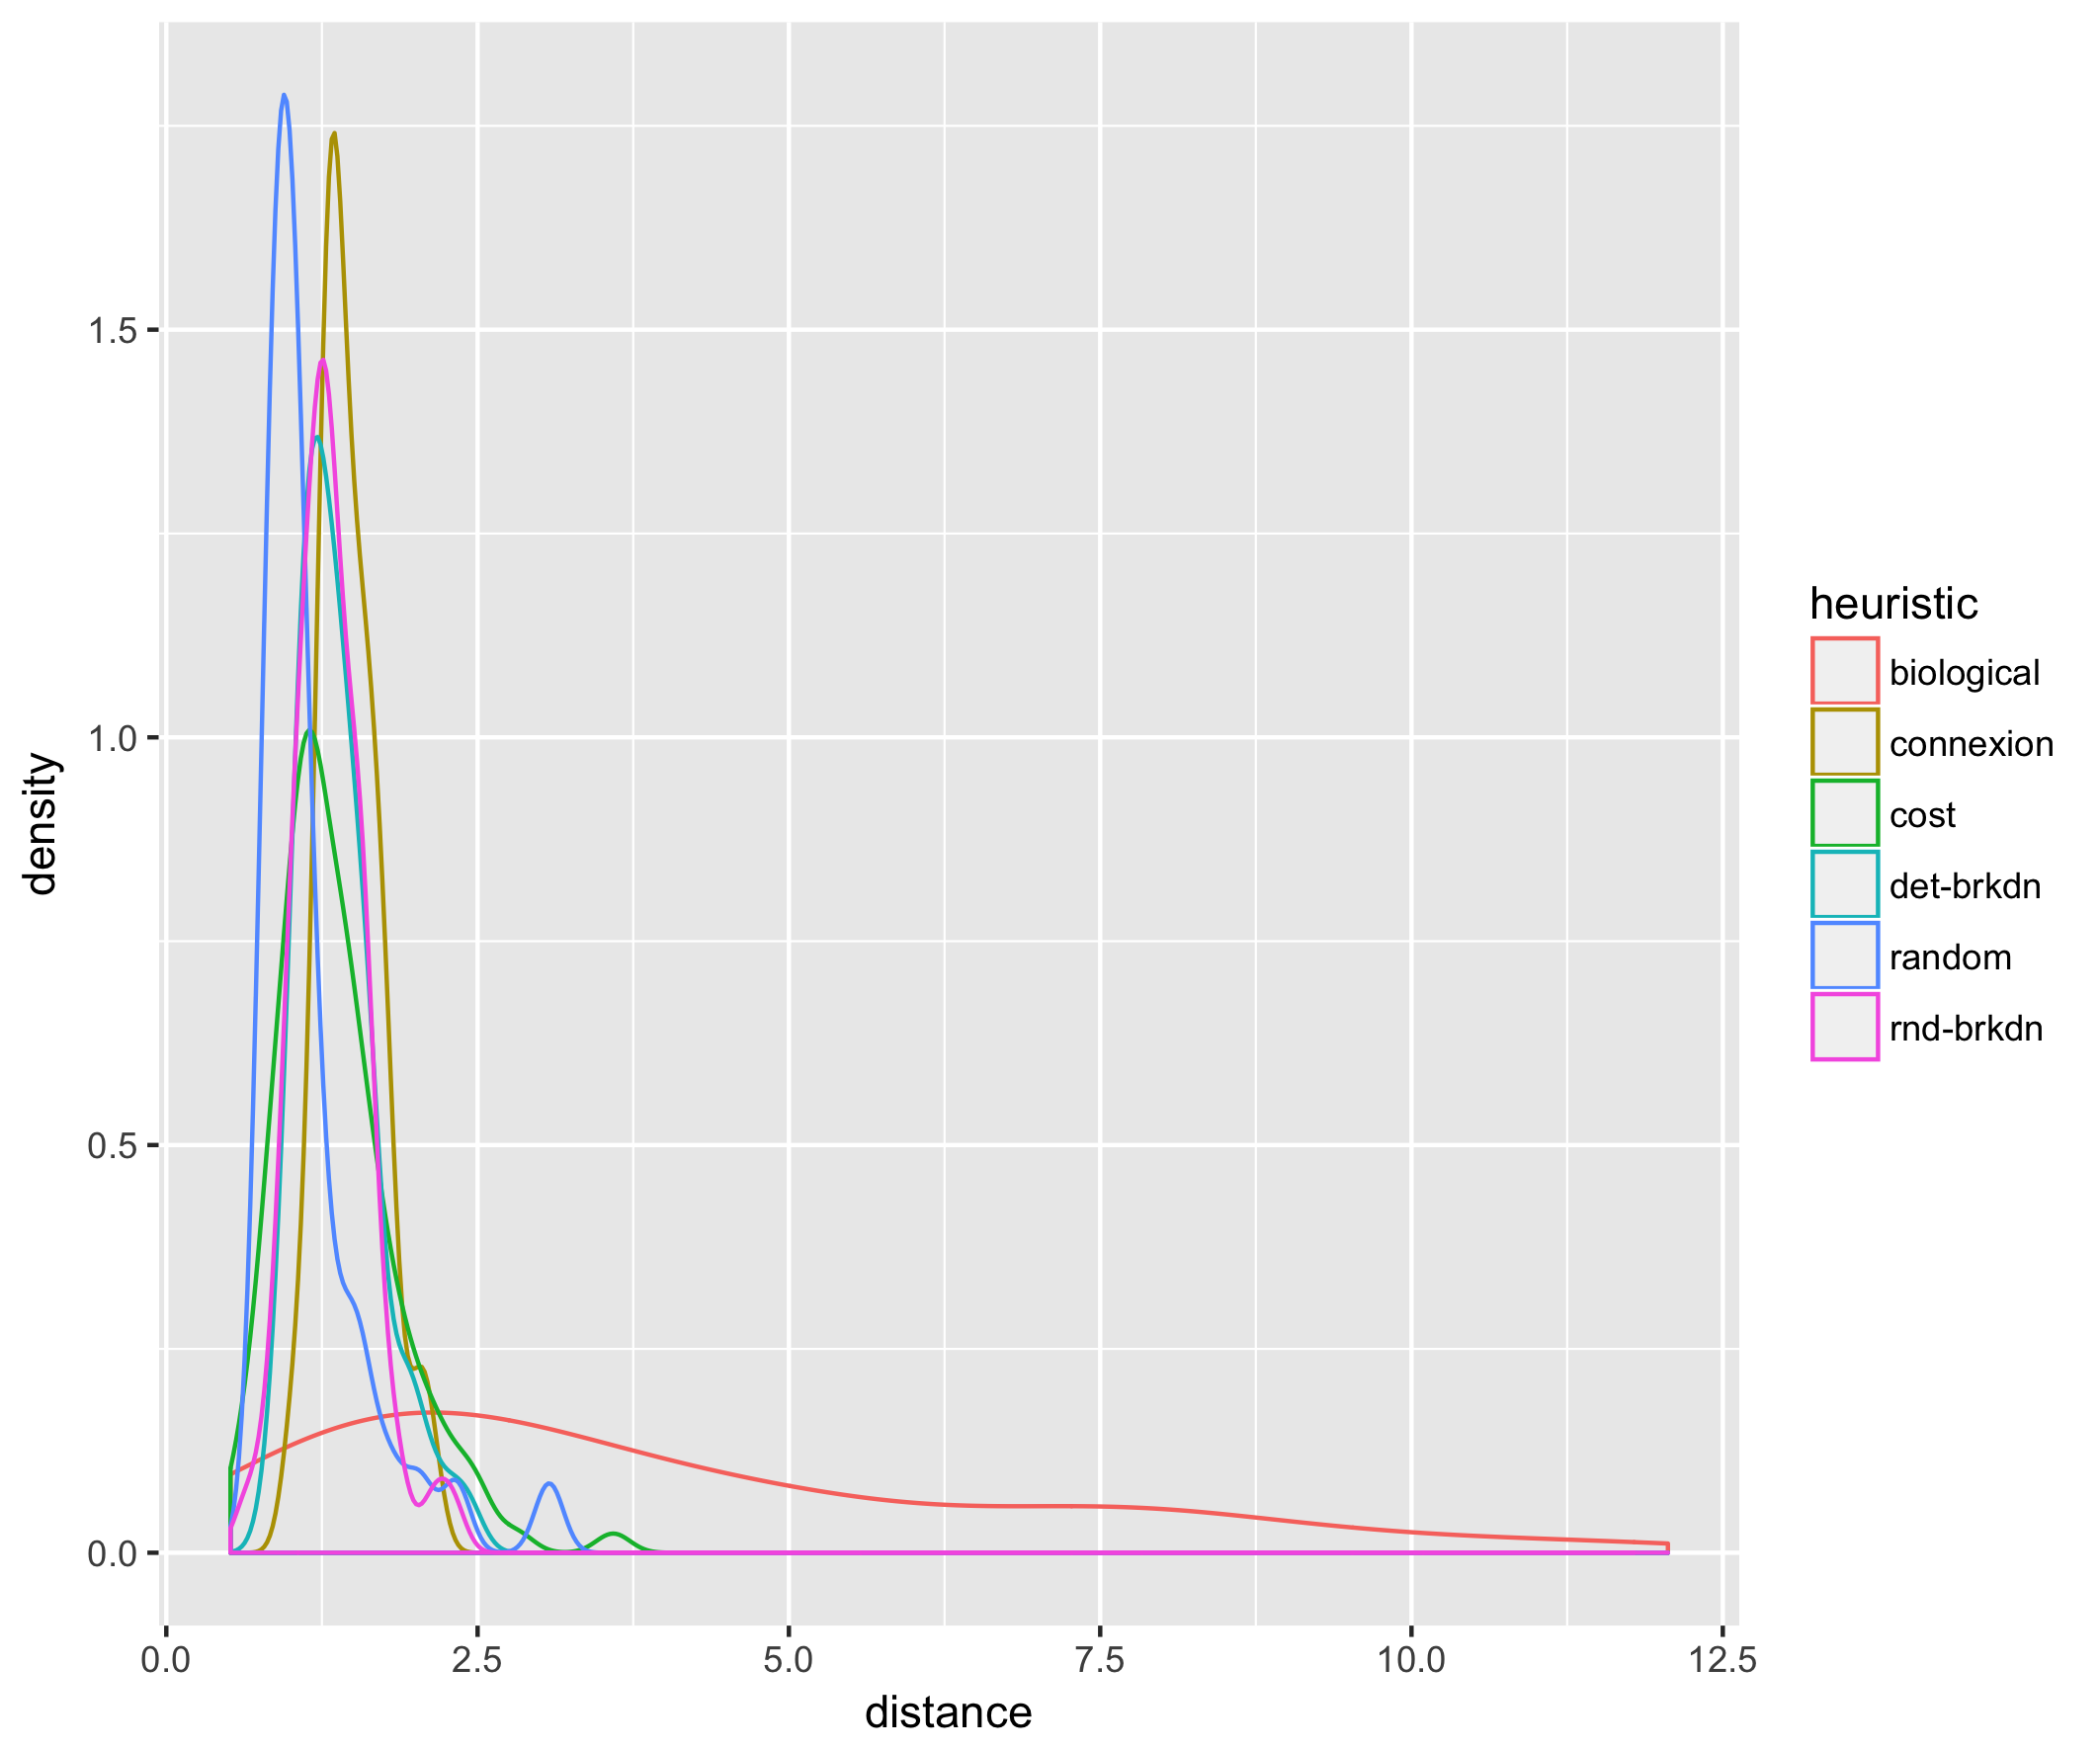
\includegraphics[width=\textwidth]{figures/coevol_corrs-distrib_rhoasize4}

\end{columns}

\footnotesize\textit{(Left) Full indicator space; (Middle) Morphological and Topology, by network heuristic; (Right) Distance distribution for cumulated distance for indicators and correlations.}

}


\sframe{Results : Causality Regimes}{

\textit{Unsupervised learning on lagged correlations between local variables unveils a diversity of causality regimes}

$\rightarrow$ Link between \emph{co-evolution regime} and morphogenetic properties of the urban system

% comment Arnaud : le genre d’affirmation qu’il faut réussir à exprimer également du point de vue de l’objet étudié : qu’est-ce que ça veut dire pour la morphogénèse urbaine ?

\medskip

\centering

\includegraphics[width=0.52\textwidth,height=0.55\textheight]{figures/coevol_centertrajs}
\includegraphics[width=0.4\textwidth,height=0.55\textheight]{figures/coevol_cluster-params}

\footnotesize\textit{(Left) Lagged correlation profiles of cluster centers; (Right) Distribution of regimes across parameter space}

}




%%%%%%%%
%% LUTECIA



%\section{Transportation Governance}
%%%%%%%%%%%%%%%%%%%



\sframe{The LUTECIA Model : Rationale}{

\justify


Towards a more complex approach to network growth rules ? $\rightarrow$ a co-evolution approach including transportation governance

\medskip

\textit{Mega-city Regions~\cite{hall2006polycentric} exhibit new qualitative regimes of urban systems ?}

\bigskip

$\rightarrow$ A LUTI + infrastructure provision model (LUTECIA)

\medskip

$\rightarrow$ Coevolution transport / urbanism (LUTI model with endogeneous transport infrastructure provision)

\medskip

$\rightarrow$ Game theory framework to predict emergence of centralized decision within a polycentric region

\medskip

$\rightarrow$ Importance of accessibility at MCR scale

}



\sframe{The LUTECIA Model : Structure}{

LU : Land Use module ; T : Transport module ; EC : Evaluation of Centralized decision module ; I : Infrastructure provision module ; A : Agglomeration economies module

\medskip

\includegraphics[width=\textwidth]{figures/lutetia_structure}

}


\sframe{Governance Modeling}{

Matrix of actors utilities, depending on respective choices

\bigskip

\begin{tabular}{ |c|c|c| } 
 \hline
 0 $|$ 1  & C & NC \\ \hline
 C & $U_i = \kappa \cdot \Delta X_i(Z^{\ast}_C) - I - \frac{J}{2}$
   & $\begin{cases}U_0 = \kappa \cdot \Delta X_0(Z^{\ast}_0)-I \\U_1 = \kappa \cdot \Delta X_1(Z^{\ast}_1)-I - \frac{J}{2}\end{cases}$ \\ \hline
 NC & $\begin{cases}U_0 = \kappa \cdot \Delta X_0(Z^{\ast}_0)-I - \frac{J}{2}\\U_1 = \kappa \cdot \Delta X_1(Z^{\ast}_1)-I\end{cases}$
   & $U_i = \kappa \cdot \Delta X_i(Z^{\ast}_i) - I$ \\
 \hline
\end{tabular}


\bigskip

Two types of games implemented :
\begin{itemize}
\item Mixed Nash equilibrium, where actors compete
\item One Rational Discrete Choice equilibrium
\end{itemize}


}




\sframe{Lutecia model parameters}{

\begin{center}
\begin{tabular}{|c|c|c|}%c|c|c|}
  \hline
 Sub-model & Parameter & Name\\% & Process & Domain & Default\\
  \hline
\multirow{5}{*}{Land-use}& $\lambda$ & Accessibility range \\\cline{2-3}% & Accessibility & $]0;1]$ & $0.001$ \\\cline{2-6}
 & $\gamma_A$ & Cobb-Douglas exponents actives\\\cline{2-3}% & \multirow{2}{*}{Utility} & $[0;1]$ & $0.85$ \\\cline{2-3}\cline{5-6}
 & $\gamma_E$ & Cobb-Douglas exponents employments \\\cline{2-3}%&  & $[0;1]$ & $0.85$ \\\cline{2-6}
 & $\beta$ & Discrete choices exponent \\\cline{2-3}%& \multirow{2}{*}{Relocalization} & $[0;+\infty]$ & $1$ \\\cline{2-3}\cline{5-6}
 & $\alpha$ & Relocation rate \\\hline%&  & $[0;1]$ & $0.05$ \\\hline
Transport & $v_G$ & Network speed \\\hline%& Hierarchy & $[1;+\infty [$ & $5$ \\\hline
\multirow{2}{*}{Governance} & $J$ & Collaboration cost\\\cline{2-3}% & \multirow{2}{*}{Planning} & $[0;0.005]$ & $0.001$ \\\cline{2-3}\cline{5-6}
 & $l_r$ & Infrastructure length \\\hline%&  & $]0;\sqrt{2}\cdot K [$ & $2$ \\\hline
\end{tabular}
\end{center}

}



\sframe{Model Output : Examples}{

\textbf{Implementation :} Netlogo ; particular treatment for dynamical programming computation of network shortest distances. Exploration with High Performance Computing on grid with \texttt{OpenMole}~\cite{reuillon2013openmole}

\medskip

\centering

\includegraphics[width=\textwidth,height=0.7\textheight]{figures/lutetia_exrun}

}


\sframe{Land-use dynamics}{

\textit{Lessons from systematic exploration of the land-use module:}

\begin{itemize}
	\item Large diversity of morphological trajectories in time for varying $\gamma_A, \gamma_E, \lambda, \beta$
	\item Diversity of final forms obtained
	\item It is possible to minimize, at fixed $\alpha = 1$, the total quantity of relocalization
\end{itemize}

\begin{center}
\includegraphics[width=0.45\textwidth]{figures/A-lutecia-morphosens.jpg}
\includegraphics[width=0.3\textwidth]{figures/A-lutecia-morphotrajs.jpg}
\end{center}

}






\sframe{Model Exploration}{

\textit{Influence of governance parameters on network topology}

\medskip
\centering

\includegraphics[height=0.8\textheight]{figures/7-3-3-fig-lutecia-governance.jpg}

}

\sframe{Model Application}{


\textit{Stylized application to the Pear River Delta Mega-city Region}

\medskip

\centering

\includegraphics[width=\textwidth]{figures/7-3-3-fig-lutecia-ex-prd.jpg}

}


\sframe{Model Application: target networks}{


\textit{Different calibration setup: current and planned network}

\medskip

\centering

\includegraphics[width=\textwidth]{figures/A-lutecia-realsetup.jpg}

}





\sframe{Model Calibration}{

\textit{Calibration on the generated network (fixed land-use)}

\medskip

\centering

\includegraphics[height=0.8\textheight]{figures/7-3-3-fig-lutecia-calib.jpg}

}


\sframe{Effects of co-evolution}{

\textit{Unveiling the coupling between urban development and transportation networks}

\medskip

\centering

\includegraphics[height=0.8\textheight]{figures/7-3-3-fig-lutecia-coevol.jpg}

}





















\sframe{What is Morphogenesis ? Examples}{

% illustrations : ants, geomorphology, neurons, self-assembly ; ARBOTRON ; paper nature aile avion
% all from netlogo library ? would be nice illustration of generative nature


% remark : do not put classical biological example to show how it has percolated to other fields

\vspace{-0.3cm}

\includegraphics[width=\textwidth,height=0.82\textheight]{figures/intro_examples}

\justify

\vspace{-0.5cm}

\footnotesize\textit{Sources (in order by column). Ants, Erosion, Game of Life: NetLogo Library ; Arbotron \cite{jun2005formation}; Industrial design \cite{Aage:2017aa}; Swarm chemistry \cite{sayama2009swarm}}
% sources : ants netlogo ; erosion netlogo ; arbotron 
%  inge : 

}





\sframe{Interdisciplinary Definition of Morphogenesis}{

% precise notions and defs

\justify

\textit{Proposition of an interdisciplinary definition}

\bigskip




\textbf{Meta-epistemological framework of imbricated notions:}

Self-organization $\supsetneq$ Morphogenesis $\supsetneq$ Autopoiesis $\supsetneq$ Life


\bigskip

\textbf{Properties:}

\begin{itemize}
\item Architecture links form and function
\item Emergence strength~\cite{bedau2002downward} increases with notion depth, as bifurcations~\cite{thom1974stabilite}
\end{itemize}

\bigskip

\textbf{Definition of Morphogenesis :} \textit{Emergence of the form and the function in a strongly coupled manner, producing an emergent architecture \cite{doursat2012morphogenetic}}



}







\sframe{Discussion}{

\justify

\vspace{-1cm}

\textbf{Implications}

(\textit{Optimisation})$\rightarrow$ Morphogenesis models (in the sense of strong links between form and function) are an appropriate tool to find optimal urban designs.

(\textit{Explication})$\rightarrow$ Simple model reproducing stylized facts: which intrinsic dimension to the urban system and its morphological aspect are effectively captured?

%$\rightarrow$ Ability to reproduce static correlations and a variety of dynamical lagged correlation regimes suggests that the model captures some of the processes of co-evolution

% implications for morphogenesis ?

\bigskip

\textbf{Developments}


$\rightarrow$ Towards dynamical calibrations ? Need of dynamical data

$\rightarrow$ Investigate the link between spatial non-stationarity and non-ergodicity

$\rightarrow$ Compare network generation models in a ``fair'' way (correcting for additional parameters, open question for models of simulation)


}



\sframe{Conclusion}{


\justify

\vspace{-1cm}

$\rightarrow$ Several morphogenesis models at the mesoscopic scale explored: \textbf{need for more coupling and comparison of models.}

\medskip

$\rightarrow$ At the macro scale of the system of cities ? \textbf{Need for multi-scale models.}

\medskip

$\rightarrow$ With more refined urban characteristics and other dimensions ? \textbf{Need for more interdisciplinarity.}

\bigskip

\footnotesize

%\textbf{References}

%Raimbault, J., Banos, A., \& Doursat, R. (2014). A hybrid network/grid model of urban morphogenesis and optimization. Proceedings of 4th ICCSA 2014. arXiv:1612.08552.

%Raimbault, J. (2017). Calibration of a Density-based Model of Urban Morphogenesis. arXiv preprint arXiv:1708.06743.

%\medskip

\textbf{Open repository} (code, data and results) at\\\texttt{https://github.com/JusteRaimbault/CityNetwork}\\
\medskip
\textbf{Acknowledgments} : We thank the \textit{European Grid Infrastructure} and its \textit{National Grid Initiatives} (\textit{France-Grilles} in particular) to give the technical support and the infrastructure.


}






\sframe{Reserve slides}{

\centering

\Large

\textbf{Reserve Slides}

}




%%%%%%%%%%%%%%%%%
%\section*{Morphogenesis}



\sframe{Morphogenesis Overview}{
% other numerous examples of fields/case of application

\cite{bourgine2010morphogenesis} : interdisciplinary workshop on morphogenesis

\bigskip

$\rightarrow$\textit{To what extent the notion is indeed transdisciplinary, i.e. are there common definitions across disciplines ? What are the concepts shared or the divergence ?}


\begin{itemize}
\item \textbf{Biology}
\begin{itemize}
\item External phenotype morphogenesis (ant colony)~\cite{minter2012morphogenesis} \item Symbiosis of species~\cite{chapman1998morphogenesis}
\item Botany~\cite{lord1981cleistogamy}
\end{itemize}
\item \textbf{Social Sciences} : Archeology~\cite{renfrew1978trajectory}
\item \textbf{Epistemology} : \cite{gilbert2003morphogenesis}
\item \textbf{Artificial Intelligence} : From self-assembly to Morphogenetic Engineering~\cite{doursat2013review}. Synthetic Biology ?
\item \textbf{Geomorphology} : dunes formation~\cite{douady2011dunes}
\item \textbf{Physics} : Arbotrons playing Tetris ?
\item etc\ldots
\end{itemize}




}



\sframe{Morphogenesis concepts}{

\begin{itemize}
\item \justify \textbf{Morphogenesis and Self-Organisation} : when does a system exhibit an architecture ? Insights from Morphogenetic Engineering
\cite{doursat2013review}. Architecture : the relation between the form and the function ?
\medskip
\end{itemize}
\begin{itemize}
\item \justify\textbf{Scales, Units and Boundaries} From local interactions to global information flow (Holland's \emph{signal and boundaries}~\cite{holland2012signals}: morphogenesis as the development of Complex Adaptive Systems ?)
\medskip
\end{itemize}
\begin{itemize}
\item \justify \textbf{Symmetry and Bifurcations} : on quantitative becoming qualitative. Ren{\'e} Thom's \emph{theory of catastrophes}~\cite{thom1974stabilite}
\medskip
\end{itemize}
\begin{itemize}
\item \justify \textbf{Life and Death} : link with autopoiesis and cognition\\
\cite{bourgine2004autopoiesis} ; co-evolution of subsystems as an alternative definition ? In psychology, attractors of the mind.
\end{itemize}


}


\sframe{Catastrophe Theory}{

% brief rapide sur theorie des catastrophes

A system is viewed as its internal state $X_w$, where $w\in W$ is a control parameter.

\bigskip

Catastrophe set $K \subset W$ is where the system endures phase transition.

\bigskip

Thom classified possible topologies for $K$ depending on the dimension of $W$.

}







%%%%%%%%%%%%%%%%%
%\section*{Co-evolution Morphogenesis}




\sframe{Defining co-evolution}{


\justify

No clear definition of co-evolution in the literature : \cite{bretagnolle:tel-00459720} distinguishes ``reciprocal adaptation'' where a sense of causality can clearly be identified, from co-evolutive regimes 


\bigskip
\bigskip

Identification of multiple causality regimes in a simple strongly coupled growth model $\rightarrow$ to be put in perspective with a theoretical definition of co-evolution based on the conjunction of Morphogenesis and the Evolutive Urban Theory

%, summarised by~\cite{raimbault2017co}

}


\sframe{Modeling Co-evolution}{

\justify

\cite{baptistemodeling} system dynamics with evolving capacities
 
\cite{wu2017city} population diffusion and network growth

\cite{blumenfeld2010network} and \cite{schmitt2014modelisation} : random potential breakdown for network growth.

\cite{barthelemy2009co} geometrical network growth model making network topology co-evolve with vertex density

}


\sframe{Empirical Data : network indicators}{

\centering

\includegraphics[width=0.9\textwidth]{figures/coevol_FR_indics_network_selected_2_discrquantiles}

}

\sframe{Empirical Data : correlations}{

\centering
\includegraphics[height=0.8\textheight]{figures/coevol_FR_corr_PCA_rhoasize12}

}



\sframe{Network Indicators}{

Network Topology measured by:

\begin{itemize}
	\item Betweenness and Closeness centralities: average and hierarchy
	\item Accessibility (weighted closeness)
	\item Efficiency (network pace relative to euclidian distance)
	\item Mean path length, diameter
\end{itemize}

}




\sframe{Model specification}{

\footnotesize

Patch utility given by $U_i = \sum_k w_k \cdot \tilde{x}_k$ with $\tilde{x}_k$ normalized local variables among population, betweenness and closeness centrality, distance to roads, accessibility ; aggregation done with probability $\left(U_i/\sum_k U_k\right)^\alpha$ ; diffusion among neighbors $n_d$ times with strength $\beta$

\medskip

\textbf{Network Generation :}

Adding a fixed number $n_N$ of new nodes : for patches such that $d_r < d_0$, probability to receive a node is

%% note : not a proba for the last ? no pb as soon as in 0,1, realized anyway.
\[
p = P/P_{max} \cdot (d_M - d)/d_M \cdot \exp\left(-((d_r - d_0)/\sigma_r)^2\right)
\]

Nodes connected the shortest way to existing network.

\medskip

\textbf{General model parameters :}

\begin{itemize}
	\item Patch utility weights $w_k$
	\item General network generation parameters: growth time steps $t_N$, maximal additional links
\end{itemize}

}



\sframe{Deterministic breakdown Network generation}{

\begin{enumerate}
\item Gravity potential given by
\[
V_{ij}(d) = \left[ (1 - k_h) + k_h \cdot \left( \frac{P_i P_j}{P^2} \right)^{\gamma} \right]\cdot \exp{\left( -\frac{d}{r_g (1 + d/d_0)} \right)}
\]

\item $k\cdot N_L$ links are selected with lowest $V_{ij}(d_N)/V_{ij}(d_{ij})$, among which $N_L$ links with highest (lest costly) are realized
\item Network is planarized
\end{enumerate}
}


\sframe{Biological Network generation}{

Adding new links with biological heuristic:

\begin{enumerate}
	\item Create network of potential new links, with existing network and randomly sampled diagonal lattice
	\item Iterate for $k$ increasing ($k\in \{ 1,2,4 \}$ in practice) :
	\begin{itemize}
		\item Using population distribution, iterate $k\cdot n_b$ times the slime mould model to compute new link capacities
		\item Delete links with capacity under $\theta_d$
		\item Keep the largest connected component
	\end{itemize}
	\item Planarize and simplify final network
\end{enumerate}

}


\sframe{Model setup}{

\textbf{Synthetic setup: } rank-sized monocentric cities, simple connection with bord nodes to avoid bord effects 

\textbf{Real setup: } Population density raster at 500m resolution (European Union, from Eurostat)

\centering
\frame{\includegraphics[width=0.35\textwidth]{figures/coevol_example_synthsetup}}\hspace{0.1cm}
\frame{\includegraphics[width=0.35\textwidth]{figures/coevol_example-realsetup}}

\textbf{Stopping conditions: } fixed final time; fixed total population; fixed network size.

}


\sframe{Calibration Method}{


%% The model is calibrated at the first order (indicators of urban form and network measures) and at the second order (correlations) with Eurostat population grid coupled with street network from OpenStreetMap through the following workflow: indicators (Moran index, mean distance, hierarchy, entropy for morphology, mean path length, centralities, performance for network) are computed on real areas of width 50km for all Europe (what corresponds to the typical scale of processes the model includes); parameter space of the model is explored using grid computing (with OpenMole model exploration software), from simple synthetic initial configurations (few connected punctual settlements), computing indicators on final simulated configurations;  among candidate parameters for given contiguous (in space and indicator space) real areas on which correlations can be computed, the one with the closest correlation matrix computed on repetitions is chosen.



\begin{itemize}
	\item Brute force exploration of a LHS sampling, 10 repetitions of the model for each parameter point.
	\item For each simulated point, closest in indicator space (euclidian distance for normalized indicators) among real points are selected.
	\item Among these, point with lowest distance to correlation matrix are taken.
\end{itemize}


}

\sframe{Calibration : optimal points}{

\centering

\includegraphics[width=0.45\textwidth]{figures/coevol_dists_pareto_i1}
\includegraphics[width=0.45\textwidth]{figures/coevol_dists_pareto_i10}

\footnotesize\textit{Pareto plots of distance to indicators and distance to correlation matrices, for a given simulated configuration and all real points.}

}



\sframe{Causality regimes: clustering}{

\centering

\includegraphics[width=0.48\textwidth]{figures/coevol_clustcoef}
\includegraphics[width=0.48\textwidth]{figures/coevol_diffclustcoef}

\medskip

\footnotesize\textit{Clustering coefficient (left) and its derivative (right) as a function of number of clusters}

}





\sframe{Co-evolution Models}{

\centering
\includegraphics[width=0.8\textwidth]{figures/thematic_coevolution}

}






\sframe{Governance Game Specification}{

Mixed Nash equilibrium probability :

\[
p_i = \frac{J}{\Delta X_{\bar{i}}{Z^{\star}_{C}} - \Delta X_{\bar{i}}{Z^{\star}_{\bar{i}}}}
\]

\medskip


% Discrete choices model

Discrete Choice model :

\[
U_i(C) - U_i(NC) = p_{\bar{i}} \left( \Delta X_{i}{Z^{\star}_{C}} - \Delta X_{i}{Z^{\star}_{i}}\right) - J
\]

then

\[
p_i = \frac{1}{1 + \exp{\left(-\beta_{DC}\cdot \left(\frac{\Delta X_{i}{Z^{\star}_{C}} - \Delta X_{i}{Z^{\star}_{i}}}{1 + \exp{\left(- \beta_{DC}(p_i \cdot (\Delta X_{\bar{i}}{Z^{\star}_{C}} - \Delta X_{\bar{i}}{Z^{\star}_{\bar{i}}}) - J)\right)}} - J \right)\right)}}
\]




}


\sframe{Lutetia : default parameter values}{

% default param values
$A_{max} = E_{max} = 500 ; r_A = 1 ; r_E = 0.8 ; \gamma_E = 0.9 ; \gamma_A = 0.65 ; \beta_{l} = 1.8 ; \lambda = 0.005 ; r_0 = 2$

$N_{expl} = 25 ; I = 0.001 ; J = 0.0001 ; \nu = 5 ; E_{ext}(t_0) = 3E_{max} ; t_f = 4$


}


\sframe{Lutetia : Land-use Initialization}{

Initial distribution of Actives and Employments around governance centers at positions $\vec{x}_i$ by
\[
A(\vec{x}) = A_{max} \cdot \exp{\left(\frac{\norm{\vec{x}-\vec{x}_i}}{r_A}\right)} ; 
E(\vec{x}) = E_{max} \cdot \exp{\left(\frac{\norm{\vec{x}-\vec{x}_i}}{r_E}\right)}
\]

}



\sframe{Lutetia : Transportation}{


Transportation module : computation of flows $\phi_{ij}$ by solving on $p_i,q_j$ by a fixed point method (Furness algorithm), the system of gravital flows
\[
\begin{cases}
\phi_{ij} = p_i q_j A_i E_j \exp{\left(-\lambda_{tr} d_{ij}\right)}\\
\sum_k \phi_{kj} = E_j ; \sum_k \phi_{ik} = A_i\\
p_i = \frac{1}{\sum_k{q_k E_k \exp{(-\lambda_{tr}d_{ik})}}} ; q_j = \frac{1}{\sum_k{p_k A_k \exp{(-\lambda_{tr}d_{kj})}}} 
\end{cases}
\]

Trajectories then attributed by effective shortest path, and corresponding congestion $c$ obtained (no Wardrop equilibrium). 

Speed of network given by BPR function $v(c) = v_0 \left(1 - \frac{c}{\kappa}\right)^{\gamma_c}$. Congestion not used in current studies (infinite capacity $\kappa$).





}



\sframe{Lutetia : Land-use Evolution}{



Land-Use module : we assume that residential/employments relocations are at equilibrium at the time scale of a tick, that corresponds to transportation infrastructure evolution time scale which is much larger (Bretagnolle, 2009).

We take a Cobb-douglas function for utilities of actives/employments at a given cell
\[
U_i (A) = X_i(A)^{\gamma_A}\cdot {F_i(A)}^{1-\gamma_A} ; F_i(A) = \frac{1}{A_i E_i}
\]
\[
U_j (E) = X_j(E)^{\gamma_E}\cdot {F_j(E)}^{1-\gamma_E} ; F_j(E) = 1
\]

where $X_i(A) = A_i\cdot \sum_j{E_j \exp{\left(-\lambda\cdot d_{ij}\right)}}$ and $X_j(E) = E_j\cdot \sum_i{A_i \exp{\left(-\lambda\cdot d_{ij}\right)}}$.

Relocations are then done deterministically following a discrete choice model :
\[
A_i(t+1) = \sum_i{A_i(t)}\cdot\frac{\exp{(\beta U_i(A))}}{\sum_i{\exp{(\beta U_i(A))}}}
\]
\[
E_j(t+1) = \sum_j{E_j(t)}\cdot\frac{\exp{(\beta U_j(E))}}{\sum_j{\exp{(\beta U_j(E))}}}
\]




}



\sframe{Lutetia : Network Distance Computation}{



Effective distances computation

\begin{itemize}
\item Euclidian distance matrix $d(i,j)$ computed analytically
\item Network shortest paths between network intersections (rasterized network) updated in a dynamic way (addition of new paths and update/change of old paths if needed when a link is added), correspondance between network patches and closest intersection also updated dynamically ; $O(N_{inters}^3)$
\item Weak component clusters and distance between clusters updated ; $O(N_{nw}^2)$
\item Network distances between network patches updated, through the heuristic of only minimal connexions between clusters ; $O(N_{nw}^2)$
\item Effective distances (taking paces/congestion into account) updated as minimum between euclidian time and $\min_{C,C'}{d(i,C)+d_{nw}(p_C(i),p_C'(j))+d(C',j)}$ ; $O(N_{clusters}^2\cdot N^2)$ [Approximed with $\min_C$ only in the implementation, consistent within the interaction ranges $\sim$ 5 patches taken in the model]. 
\end{itemize}


}








%%%%%%%%%%%%%%%%%%%%%
\begin{frame}[allowframebreaks]
\frametitle{References}
\bibliographystyle{apalike}
\bibliography{/Users/juste/ComplexSystems/CityNetwork/Biblio/Bibtex/CityNetwork,biblio,biblio_morphogen,dynamite,ccupd,projetCSMS}
\end{frame}
%%%%%%%%%%%%%%%%%%%%%%%%%%%%
%ccupd,global,projetCSMS,dynamite



\end{document}







